\documentclass{article}

\usepackage[T1]{fontenc}    %Schriftart des Dokumentes
\usepackage[ngerman]{babel} %Dokumentensprache, hier Deutsch
\usepackage{amsmath, amssymb, stmaryrd} %mathematische Schriftzeichen
\usepackage{graphicx} %Einfügen von Grafiken
\usepackage{wrapfig}
\usepackage{bm}
\usepackage{subfig}
\usepackage{newclude}
\usepackage{pdfpages}
\usepackage{hyperref}
\hypersetup{
    colorlinks,
    citecolor=black,
    filecolor=black,
    linkcolor=black,
    urlcolor=black
}

\makeatletter
\newcommand\invisiblesection[1]{%
  \refstepcounter{section}%
  \addcontentsline{toc}{section}{\protect\numberline{\thesection}#1}%
  \sectionmark{#1}\phantom{}}
\makeatother

\setlength{\parindent}{0pt} %Einrückung von Absätzen auf null gesetzt
\setlength{\parskip}{10pt} %Abstand zischen Absätzen auf 10pt gesetzt

\title{Versuch 241: Wechselstromeigenschaften von RLC-Gliedern}
\author{Matthias Kuntz}
\date{06. \& 13.05.2024}

\renewcommand*\contentsname{Zusammenfassung}

\begin{document}

\maketitle

\tableofcontents

\newpage

%-------------------------EINLEITUNG-------------------------
\section{Einleitung}

In diesem Versuch soll es um die Grundlagen von einfachen Schaltkreisen bestehend aus ohmschen Widerständen, Kapazitäten und Spulen gehen. Dabei betrachten wir sowohl Gleich- als auch Wechselspannung sowie in einem Versuchsteil sogar komplexere Spannungssignale. Es werden verschiedene Messungen physikalischer Größen wie der Zeitkonstante, Resonanzfrequenz oder Dämpfungskonstante durchgeführt und diese mit den theoretisch zu erwartenden Werten verglichen. Zudem werden Aufnahmen verschiedener Frequenzgänge qualitativ und quantitativ analysiert und ausgewertet, was im Endeffekt zu einem besseren Verständnis der zugrundeliegenden Theorie sowie den Funktionsweisen verschiedener Schaltungen führen soll.


\subsection{Physikalische Grundlagen}

\subsubsection{Einfaches RC-Glied bei Gleichspannung}

Betrachtet man einen einfachen Schaltkreis bestehend aus einer Gleichspannungsquelle $U_E$, einem ohmschen Widerstand $R$ sowie einer Kapazität $C$ in Reihe geschaltet, so kann man den zeitlichen Verlauf der Spannung über dem Kondensator folgendermaßen betrachten: Beginnt Strom zu fließen, so lädt sich der Kondersator langsam mit der Spannung $U_C$ auf bis diese die Eingangsspannung erreicht. Mathematisch wird der Ladevorgang über die Kirchoff'sche Maschenregel folgendermaßen beschrieben:

\begin{equation}
    U_E = U_C + U_R = U_C + IR = U_C + \dot{Q} R = U_C + RC \ \dot{U}_C.
\end{equation}

Dies ist eine inhomogene Differentialgleichung erster Ordnung. Definiert man die Zeitkonstante $\tau = RC$ kann man unter der Annahme, dass der Ladevorgang bei $t=0$ beginnt, die folgende elementare Lösung finden:

\begin{equation}
    U_C (t) = U_E \cdot ( 1 - e^{-t/\tau}).
\end{equation}

Hierbei bestimmt die Zeitkonstante das zeitliche Verhalten und sie kann durch Messung der Halbwertszeit $T_{1/2}$ der Kondensatorspannung berechnet werden:

\begin{equation}
    \begin{split}
        \frac{U_E}{2} &= U_E \cdot ( 1 - e^{-T_{1/2}/\tau}) \\
        &\Rightarrow \tau = \frac{T_{1/2}}{\ln{2}}
    \end{split}
    \label{eq:E_zeitkonst}
\end{equation}

Wird keine Gleichspannung sondern beispielsweise ein Rechtecksignal an den Schaltkreis angeschlossen, so kann man ein durch die Zeitkonstante bestimmtes Wechseln von Lade- und Entladevorgängen beobachten. 


\subsubsection{Impedanz}

Es sollen kurz die Wechselstromwiderstände $Z$ (Impedanzen) der drei verwendeten Bauteile ohmscher Widerstand $R$, Kapazität $C$ und Spule $L$ genannt werden. Diese ergeben sich aus dem Verhältnis der Spannung $U(t)$ zum Stromfluss $I(t)$ über dem jeweiligen Bauteil folgendermaßen:

\begin{equation}
    \begin{split}
        Z_R &= R \\
        Z_C &= - \frac{i}{\omega C} \\
        Z_L &= i \omega L
    \end{split}
\end{equation}

\subsubsection{RC-GLieder im Wechselstromkreis}

Betreibt man die im ersten Kapitel erläuterte Schaltung mit einer Wechselspannung und beobachtet wieder den Spannungverlauf über dem Kondensator, so muss nun dessen Impedanz $Z_C$ berücksichtigt werden:

\begin{equation}
    \begin{split}
        U_C(t) &= \frac{Z_C}{R + Z_C} U_E(t) = \frac{- i /(\omega C)}{ R - i /(\omega C)} U_0 \ e^{1 \omega t} \\ 
        \Rightarrow |U_C| &= \frac{|U_E|}{\sqrt{1+ (\omega R C)^2}}
    \end{split}
\end{equation}

Der Betrag der Spannung verhält sich hierbei wie ein Tiefpassfilter, da er füh hohe Frequenzen $\omega$ abnimmt und für $\omega \xrightarrow{} 0$ gegen $|U_E|$ geht. Zusätzlich beobachtet man eine frequenzabhängige Phasenverschiebung zwischen Eingangs- und Ausgangssignal. Vertauscht man Kondensator und Widerstand und misst die Spannung über dem Widerstand $U_R$, so beobachtet man ein Hochpassverhalten:

\begin{equation}
    |U_R| = \frac{|U_E|}{\sqrt{1+ 1/(\omega R C)^2}}
\end{equation}

Eine wichtige Größe ist hier die Grenzfrequenz $\omega_g$, die angibt, bei welcher Frequenz das Eingangssignal auf das 1/$\sqrt{2}$ - fache angestiegen bzw. abgefallen ist:

\begin{equation}
    \omega_g = \frac{1}{RC} = \frac{1}{\tau}
\end{equation}

\subsubsection{RC-Glied als Integrator und Differentiator}

Wählt man die Komponenten eines RC-Glieds so, dass $\tau \gg T$ gilt, wobei $T$ die Periodendauer des Signals ist, so entspricht das Ausgangssignal $U_A$ dem Integral des Einganssignals $U_E$. Entsprechen gilt umgekehrt bei $\tau \ll T$, dass das Ausgangssignal der Ableitung des Eingangssignals entspricht. Im ersten Fall spricht man von einem Integrator, im Zweiten von einem Differentiator. Da in diesem Versuch nur qualitative Beobachtungen zu diesem Aspekt gemacht werden ist die Herleitung hier nicht weiter interessant und wird dem Umfang zuwillen ausgelassen.

\subsubsection{Elektrischer Schwingkreis (RLC-GLied)}

Eine Schaltung aus Kondensator und Spule wird Schwingkreis genannt, da sich die beiden Bauteile aufgrund ihrer physikalischen Bauweise immer wieder gegnseitig entladen und beladen, wodurch eine sinusförmige Oszillation der Spannung über diesen beobachtbar ist. Bei einer Reihenschaltung von ohmschem Widerstand $R$, Induktivität $L$ und Kapazität $C$ ergibt sich die folgende mathematische Beschreibung über die Maschenregel:

\begin{equation}
    \begin{split}
        U_R + U_C - U_L = 0 \\
        \Rightarrow L \frac{d^2}{dt^2} I + R \frac{d}{dt^2} I + \frac{1}{C} I = 0
    \end{split}
\end{equation}

Wenn der ohmsche Widerstand verschwindet, $R=0$, so ist der Schwingkreis ungedämpft und oszilliert sinusförmig mit der Eigenfrequenz

\begin{equation}
    \omega_0 = \frac{1}{\sqrt{LC}}.
\end{equation}

Ist jedoch ein Widerstand $R > 0$ vorhanden so erhalten wir einen gedämpften Schwinkreis, dessen allgemeine Beschreibung recht komplex ist, weshalb wir uns hier auf den sogenannten Schwingfall mit schwacher Dämpfung beschränken, bei dem die Amplitude mit der Zeit exponentiell abnimmt. In diesem Fall ergibt sich für die Frequenz des gedämpften Schwingkreises

\begin{equation}
    \omega_f = \sqrt{\frac{1}{LC} - \frac{R^2}{4L^2}},
    \label{eq:GedämpfterSchwingkreis}
\end{equation}

was stets kleiner als die Frequenz $\omega_0$ des freien Oszillators ist. 

Wie bereits erwäht sinkt die Amplitude proportinal zu $e^{-\delta t}$, wobei die Dämpfungskonstante $\delta$ die Abnahme bestimmt. Sie ist zusätzlich der Kehrwert zur Relaxionszeit bzw. Abklingzeit $\tau_r$:

\begin{equation}
    \delta = \frac{R}{2L} = \frac{1}{\tau_r}  .
\end{equation}

Die Abnahme der Amplituden zweier benachbarter Peaks $A_n$ und $A_{n+1}$ kann auch mit dem sogenannten logarithmischen Dekrement $\Lambda$ und darüber mit der Dämpfungskonstante in Verbindung gebracht werden:

\begin{equation}
    \Lambda = \ln{\left( \frac{A_n}{A_{n+1}} \right)} = \delta T.
\end{equation}

\subsubsection{Frequenzabhängigkeit des Schwingkreises und Resonanz}

Wird der Schwingkreis von außen mit einer Frequenz angeregt, so übernimmt dieser, wie im klassisch mechanischen Fall, nach einiger Zeit die anregende Frequenz. Aus der Gesamtimpedanz $Z_g = Z_R + Z_C + Z_L$ lässt sich der Gesamtstrom im Schwingkreis mithilfe des Ohmschen Gesetzes $I = U_E / Z_g$ berechnen:

\begin{equation}
    \begin{split}
        I(t) &= \frac{1}{R + i (\omega L - 1/(\omega C))} U_0 \ e^{i (\omega t - \phi)} \\
        \Rightarrow |I(\omega)| &= \frac{|U_0|}{\sqrt{R^2 + (\omega L - 1/(\omega C))^2}}
    \end{split}
\end{equation}

Diese Amplitude wird maximal bei der Resonanzfrequenz

\begin{equation}
    \omega_R = \sqrt{\frac{1}{LC}},
\end{equation}

bei der der Strom im Schwingkreis einfach $I(\omega_R) = U_0 / R$ entspricht und Strom und Spannung in Phase sind. Man kann nun die Amplitude der Spannung über die einzelnen Bauteile gemäß $|U| = |Z|/|I|$ berechnen. Hierbei ergibt sich:

\begin{equation}
    \begin{split}
        |U_R| &= \frac{R}{\sqrt{R^2 + (\omega L - 1/(\omega C))^2}} U_0, \\
        |U_C| &= \frac{1/(\omega C)}{\sqrt{R^2 + (\omega L - 1/(\omega C))^2}} U_0, \\
        |U_L| &= \frac{\omega L}{\sqrt{R^2 + (\omega L - 1/(\omega C))^2}} U_0. \\
    \end{split}
\end{equation}

Es ergibt sich ein sogenanntes Bandpassverhalten, bei dem die Amplituden bei einer Resonanzfrequenz maximal werden und etwa der Eingangsamplitude entsprechen, dafür aber bei anderen Frequenzen gedämpft werden. Aufgrund der leicht unterschiedlichen Formen ergeben sich auch leicht unterschiedliche Resonanzfrequenzen. Die des ohmschen Widerstands entspricht noch dem vorherigen Fall, jedoch unterscheiden sich die anderen leicht:

\begin{equation}
    \begin{split}
        \omega_C &= \sqrt{\omega_R^2 - 2\delta^2}, \\
        \omega_L &= \sqrt{\omega_R^2 + 2\delta^2}. \\
    \end{split}
\end{equation}

Bei diesen beiden Bauteilen tritt auch das Phänomen der Resonanzüberhöhung auf, bei dem die Amplitude der Spannung bei der Resonanzfrequenz deutlich höher ist als die Eingangsamplitude. 


\subsubsection{Resonanzkurven im Parallelschwingkreis}

Betrachtet man nun den Fall, in dem ein Schwingkreis aus einer Parallelschaltung von Kapazität und Widerstand aufgebaut ist, welche danach in Reihe mit einem ohmschen Widerstand verbunden ist über welchen die Spannung gemessen wird, so ergibt sich das praktisch umgekehrte Bild, bei dem im Resonanzfall die Spannung über dem ohmschem Widerstand verschwindet und der LC-Kreis eine gegen unendlich gehende Impedanz aufweist. Dieses Verhalten wird auch als Isolator bezeichnet. Die Resonanzfrequenz ergibt sich hier erneut als

\begin{equation}
    \omega_0 = \frac{1}{\sqrt{LC}}.
\end{equation}

\newpage
\subsection{Versuchsaufbau}

Herzstück des Aufbaus ist ein Steckbrett, auf welches verschiedenste Widerstände, Kapazitäten, Spulen und andere Bauteile gesteckt werden können. Betrieben und ausgemessen wird das ganze von einem digitalen Frequenzgenerator und Speicheroszilloskop, welches mit der PC-Software 'CASSY Lab 2' betrieben wird. Ein zusätzlicher Impedanzwandler dient dem Ausgleich des Innenwiderstands des Funktionsgenerators, sodass dieser über die vielen verschiedenen Konfigurationen des Versuchs ein konstantes Verhalten aufzeigt. Die Software dient auch gleichzeitig zum Abspeichern der Messdaten sowie von Bildern der Messungen, welche nach dem Messprotokoll zu sehen sind. 

Während dem Versuch werden also immer auf dem Steckbrett die richtigen Schaltkreise aufgebaut, diese über den Funktionsgenerator mit einer Spannungsquelle versehen und die Spannungen über einzelne Bauteile mit dem Oszilloskop vermessen.


\phantom{.}

\begin{figure}[!h]
    \centering
    \resizebox{0.9\textwidth}{!}{
    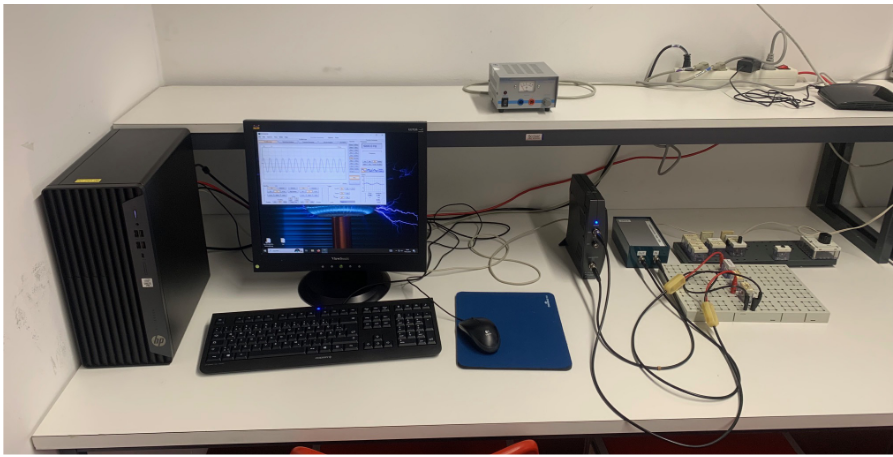
\includegraphics{graphics/aufbau.png}}
    \caption{Versuchsaufbau [Quelle: PAP2.2 Skript, S.2, Stand: 09.06.2024]}
    \label{fig:Aufbau}
\end{figure}




%---------------VERSUCHSPROTOKOLL MIT MESSDATEN---------------
\newpage

\section{Versuchsprotokoll mit Messdaten}

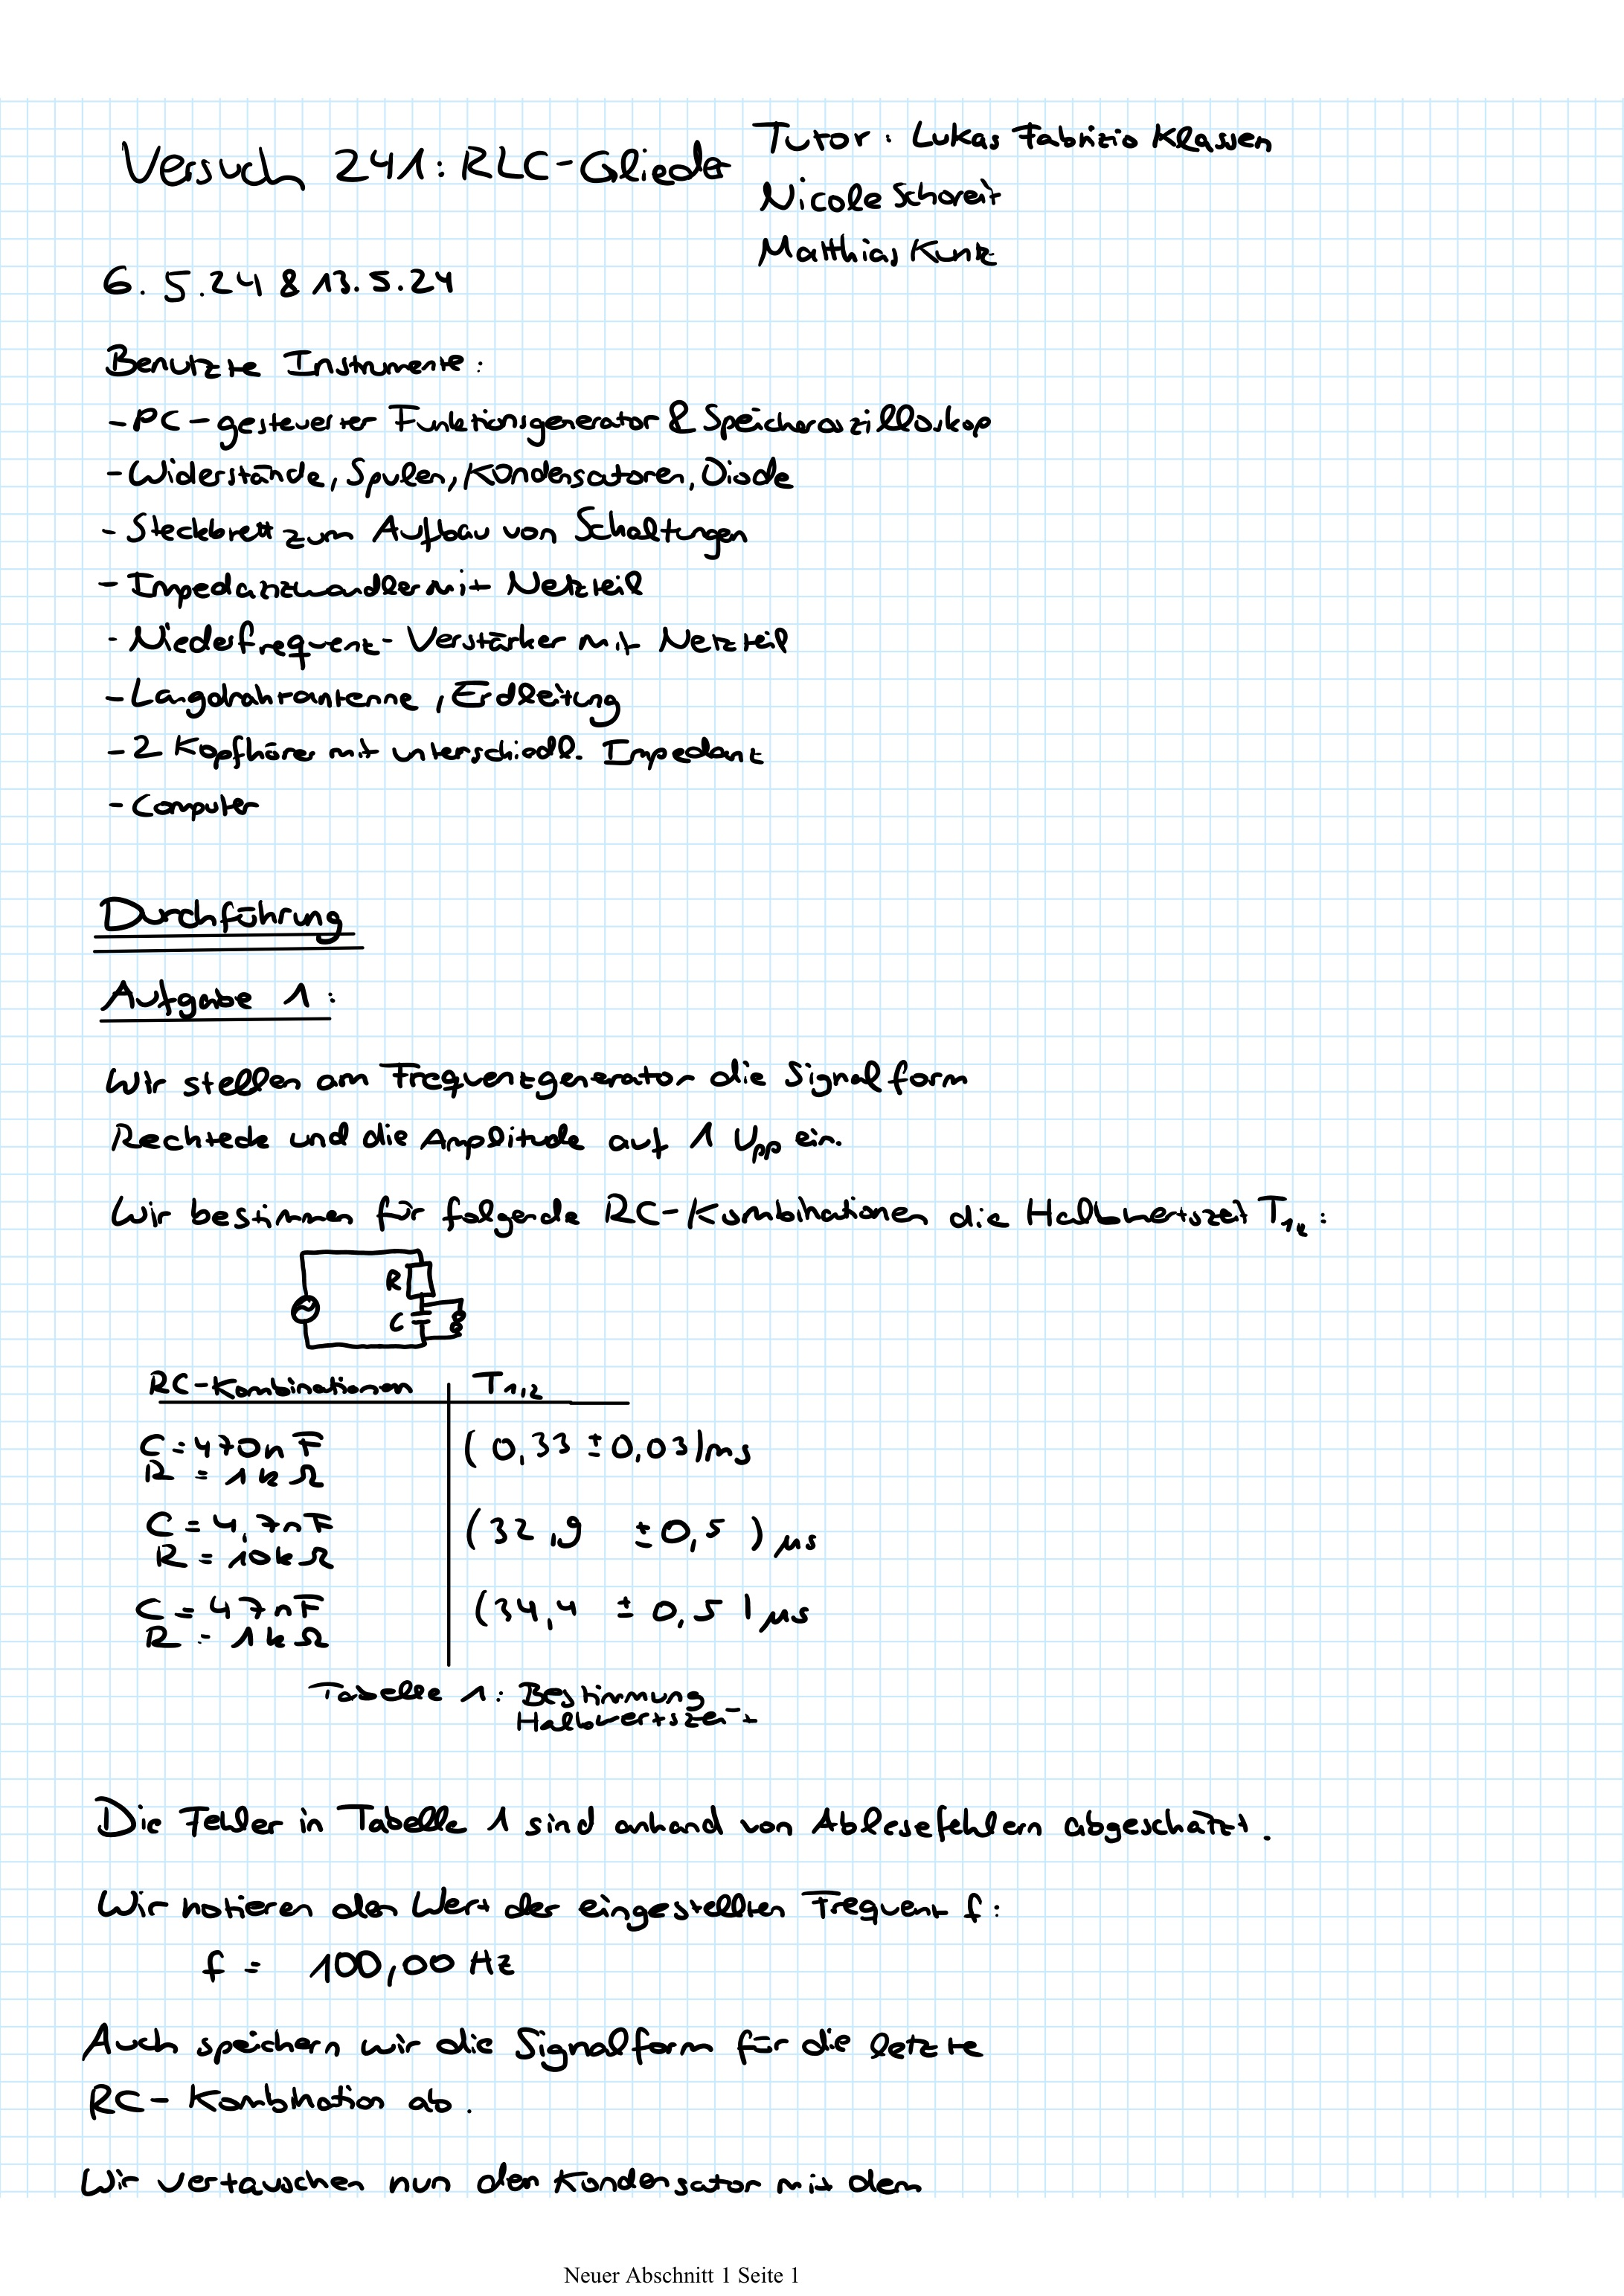
\includegraphics[width=\textwidth]{graphics/mess1.jpg}
\newpage
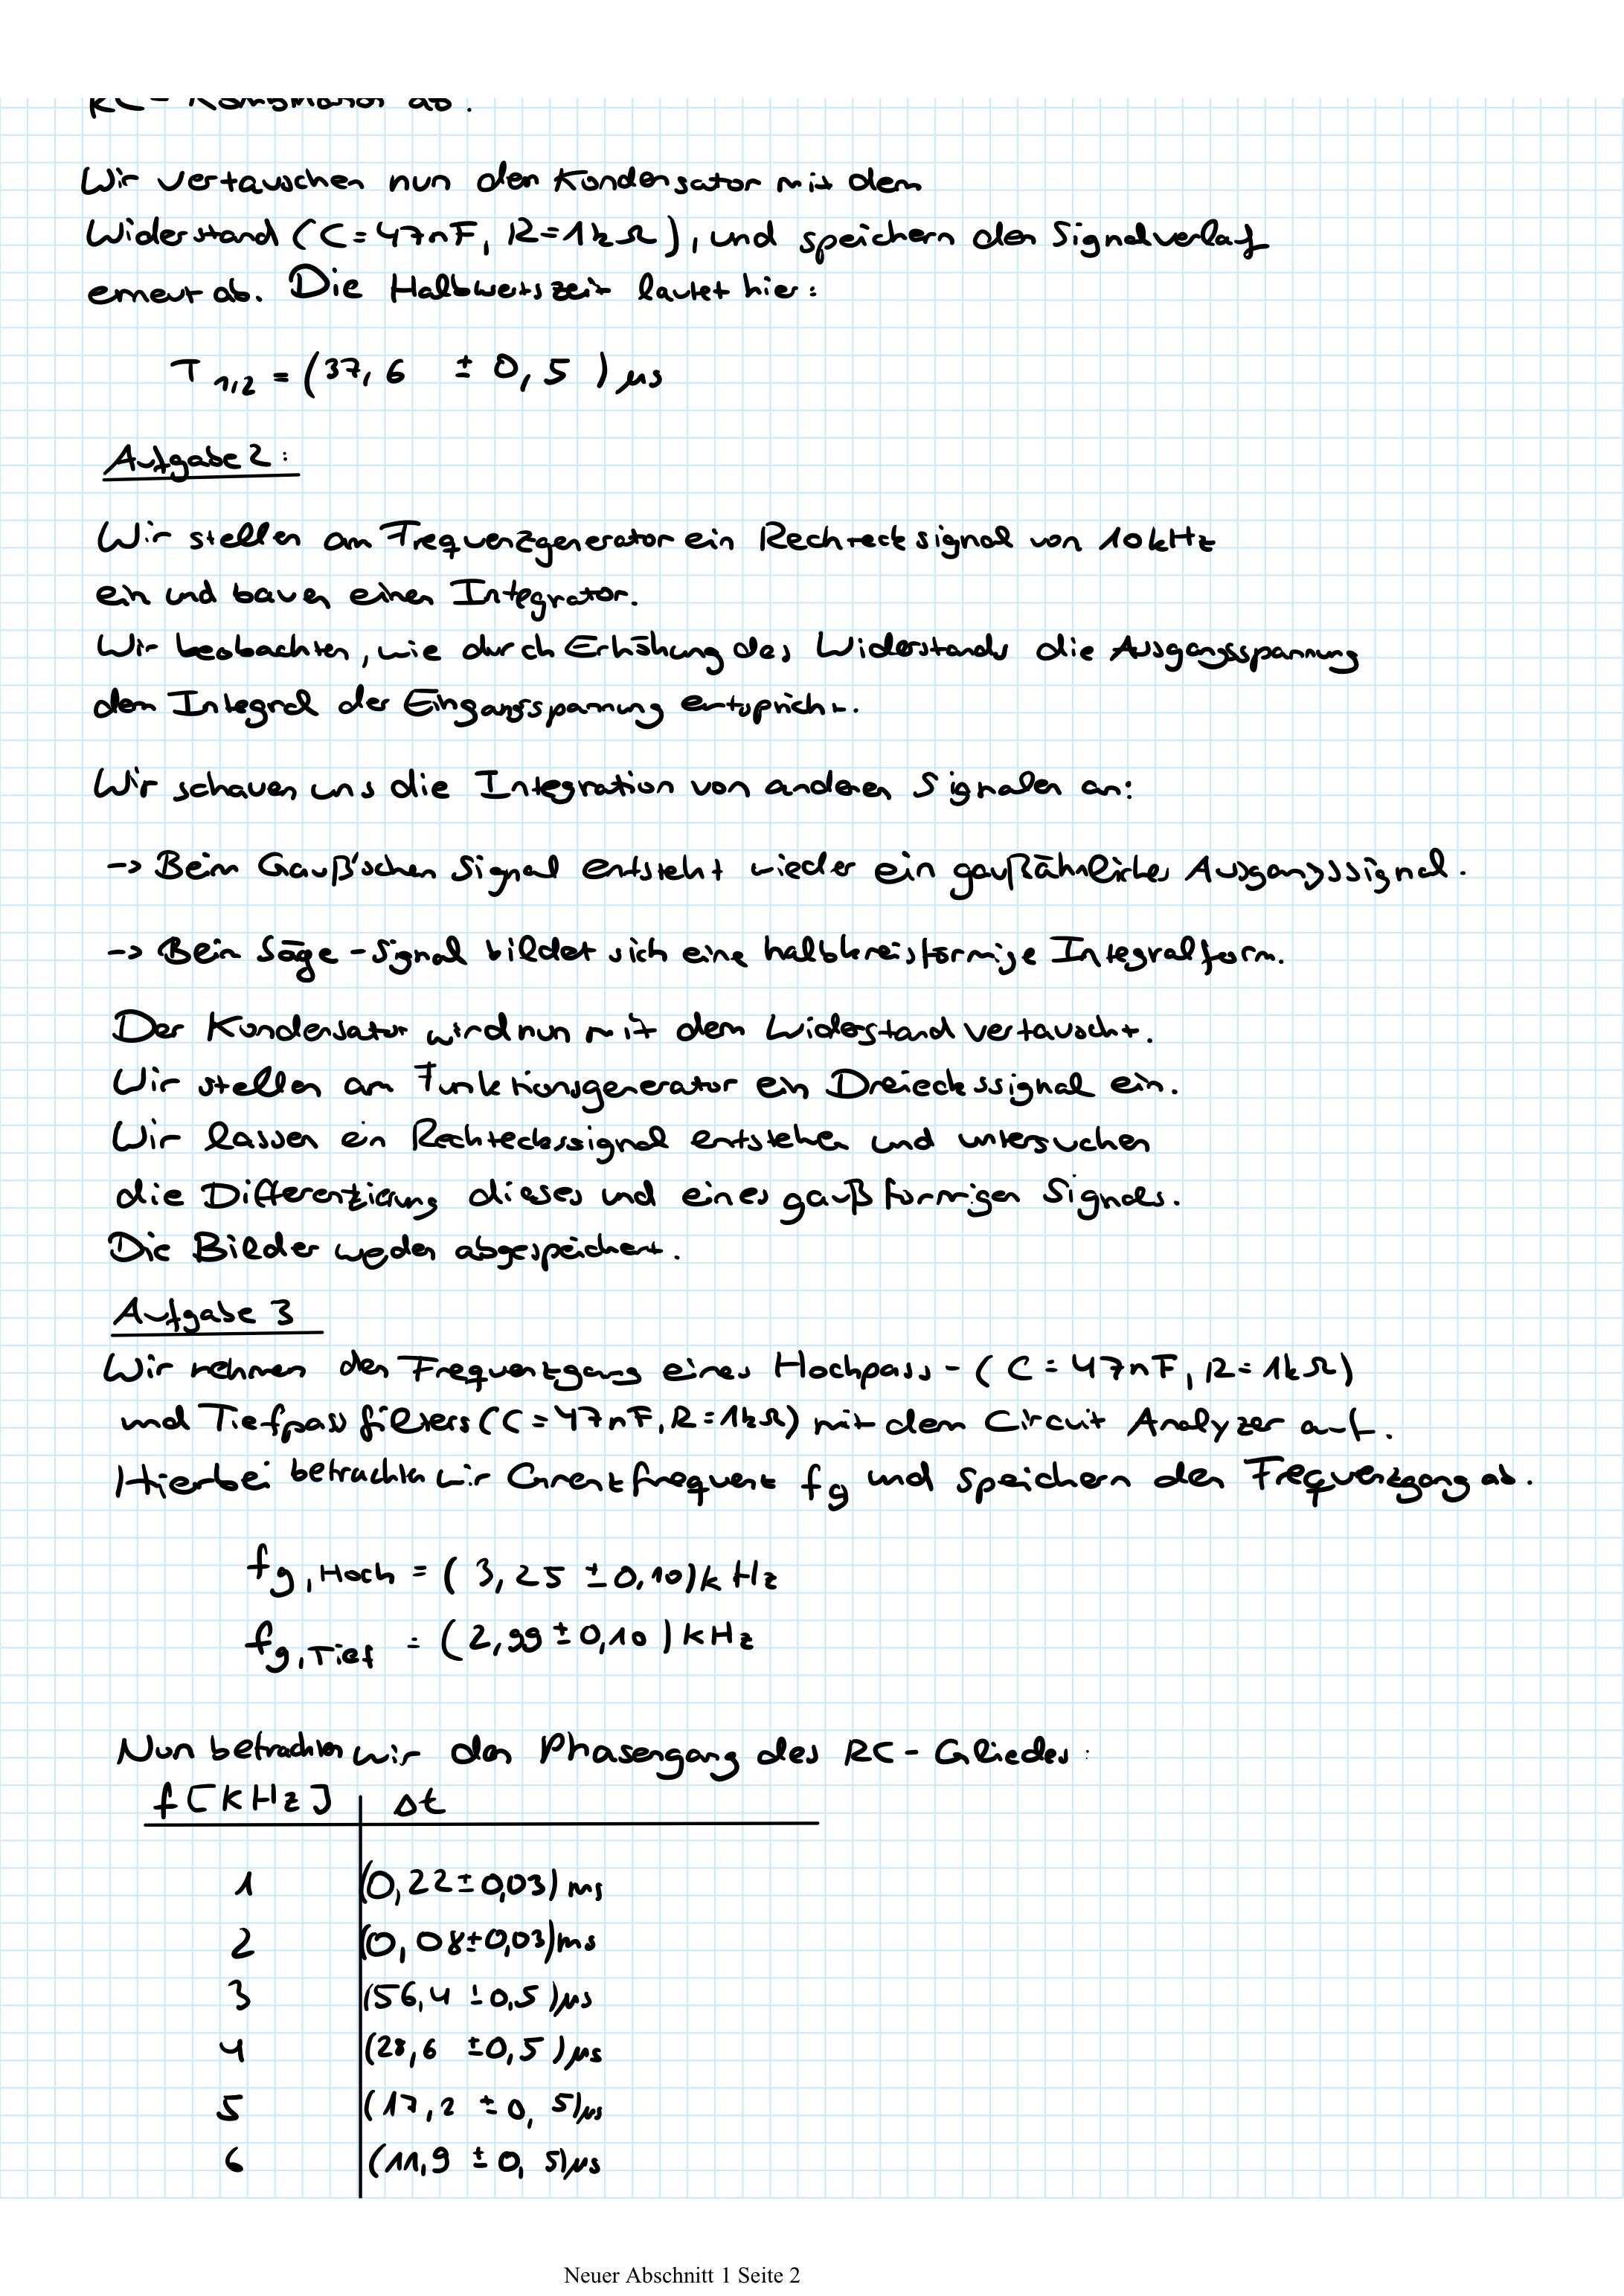
\includegraphics[width=\textwidth]{graphics/mess2.jpg}
\newpage
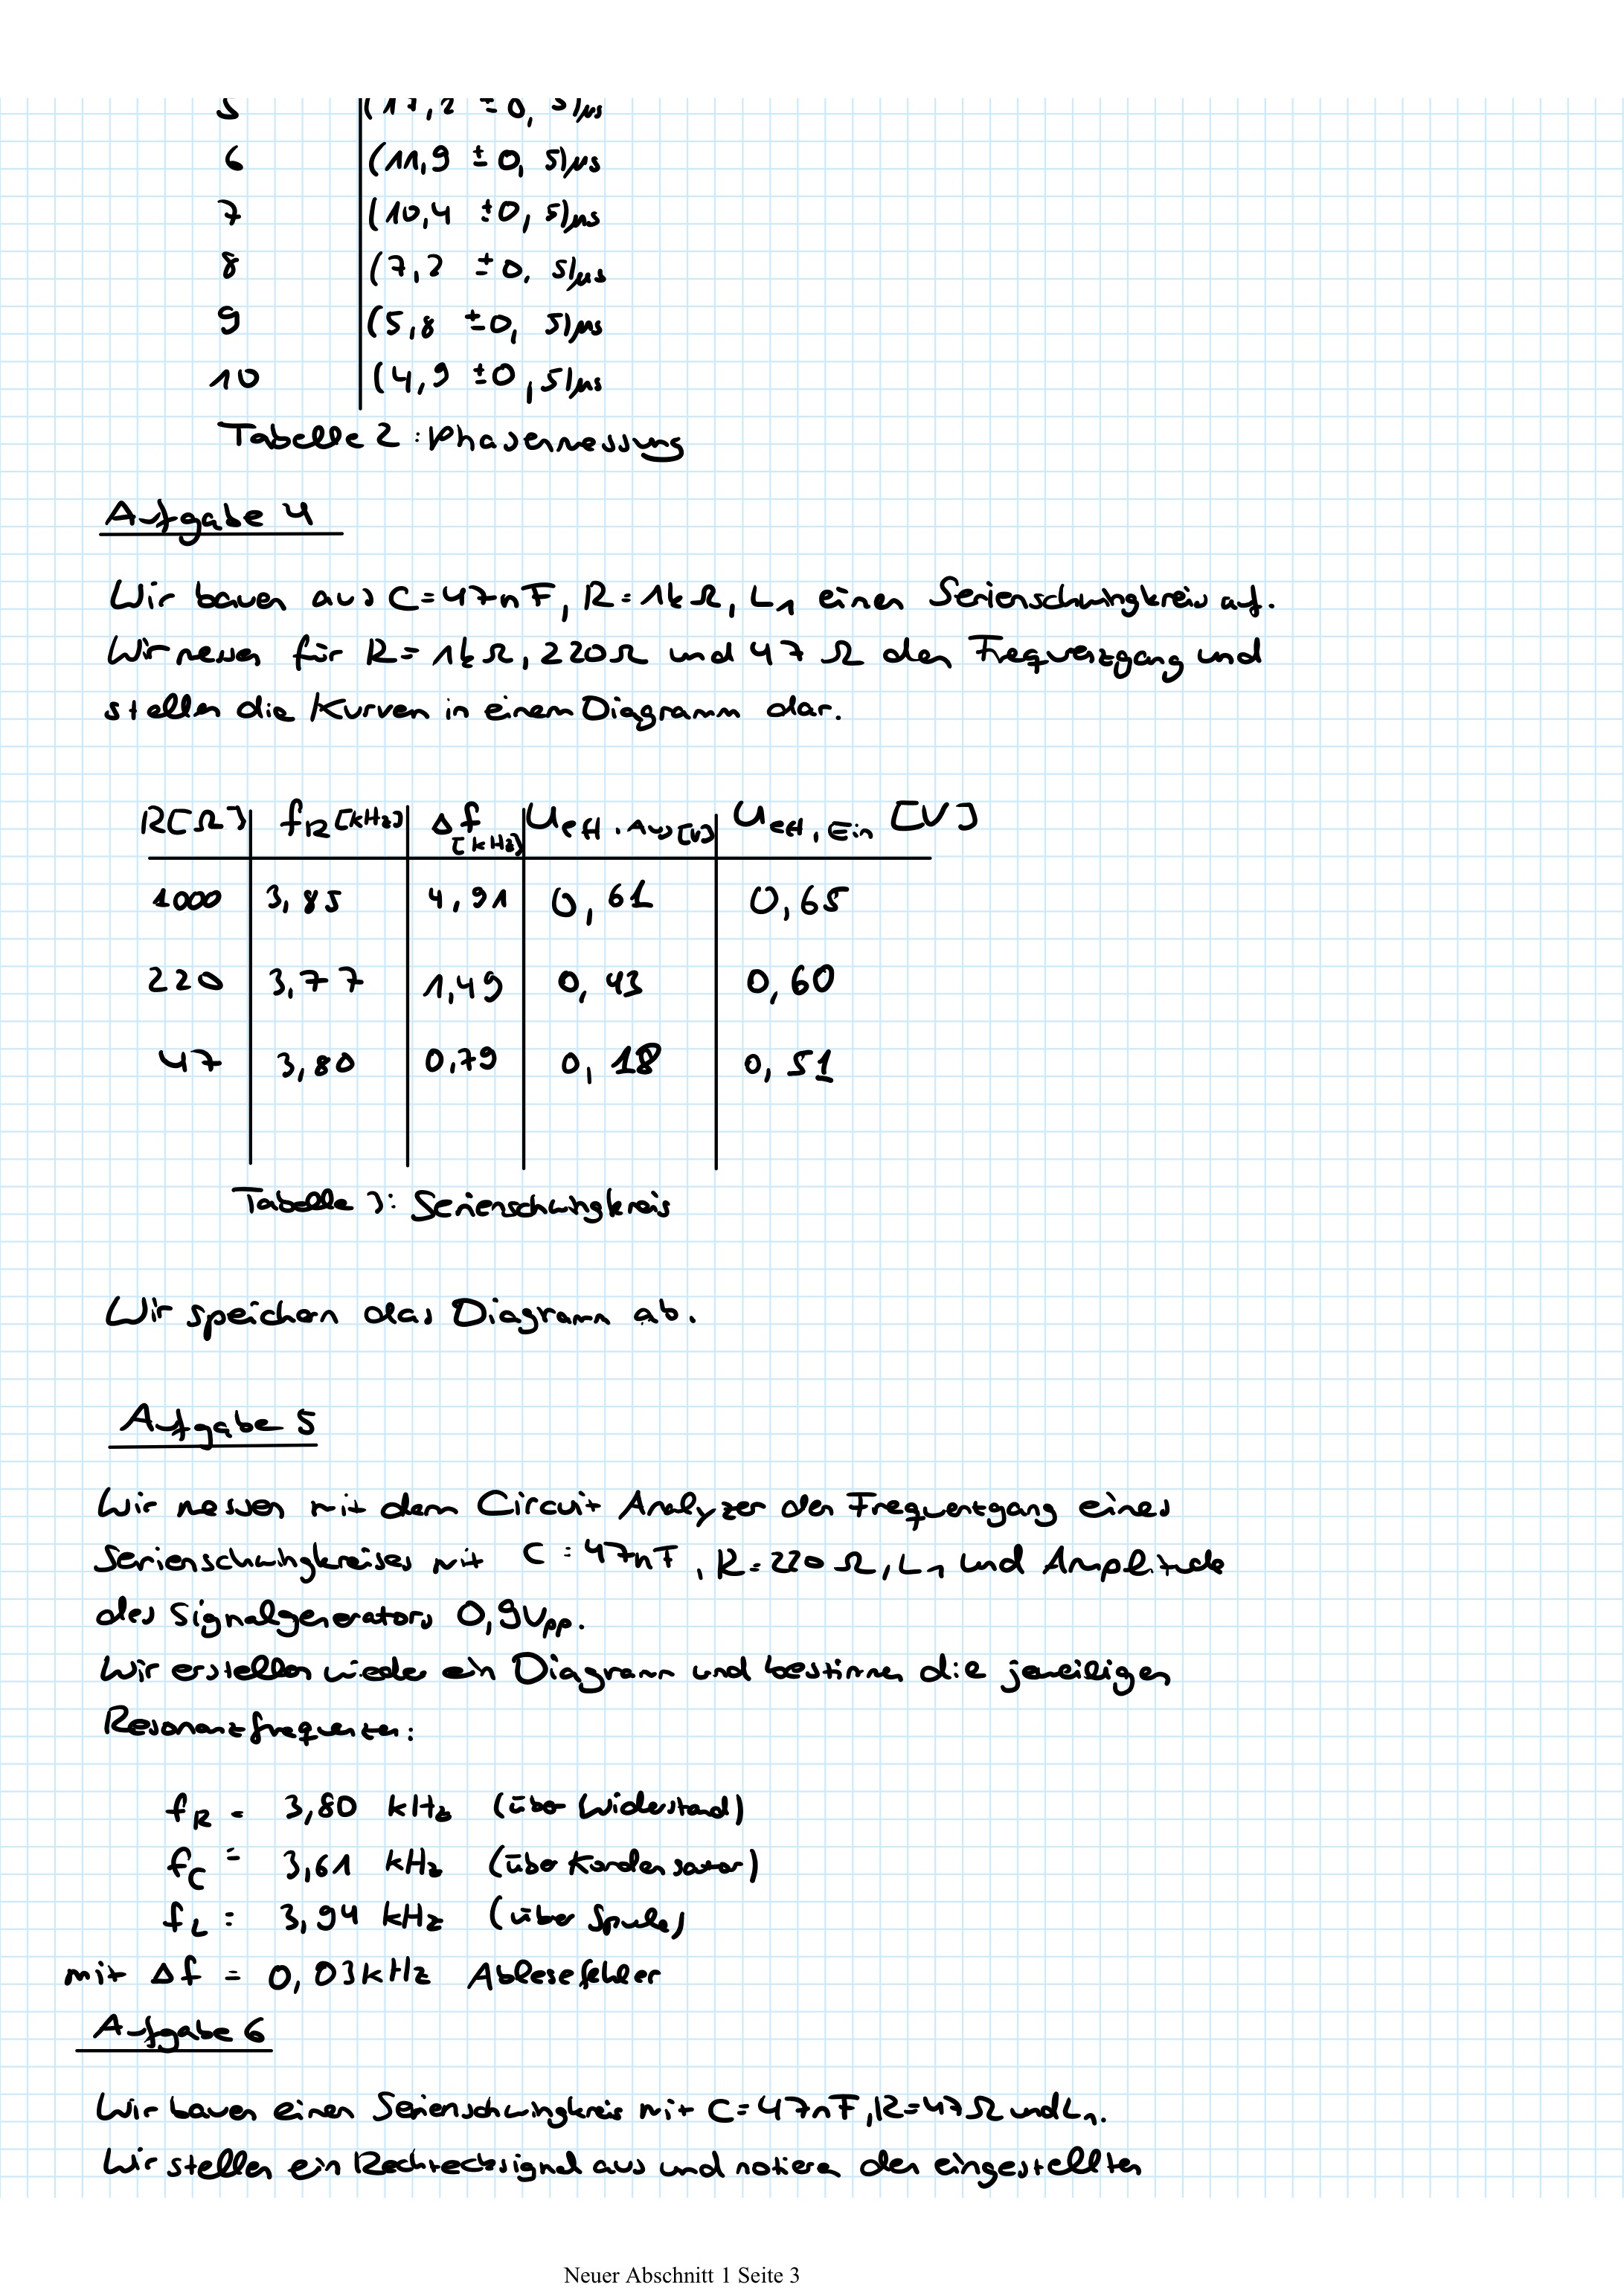
\includegraphics[width=\textwidth]{graphics/mess3.jpg}
\newpage
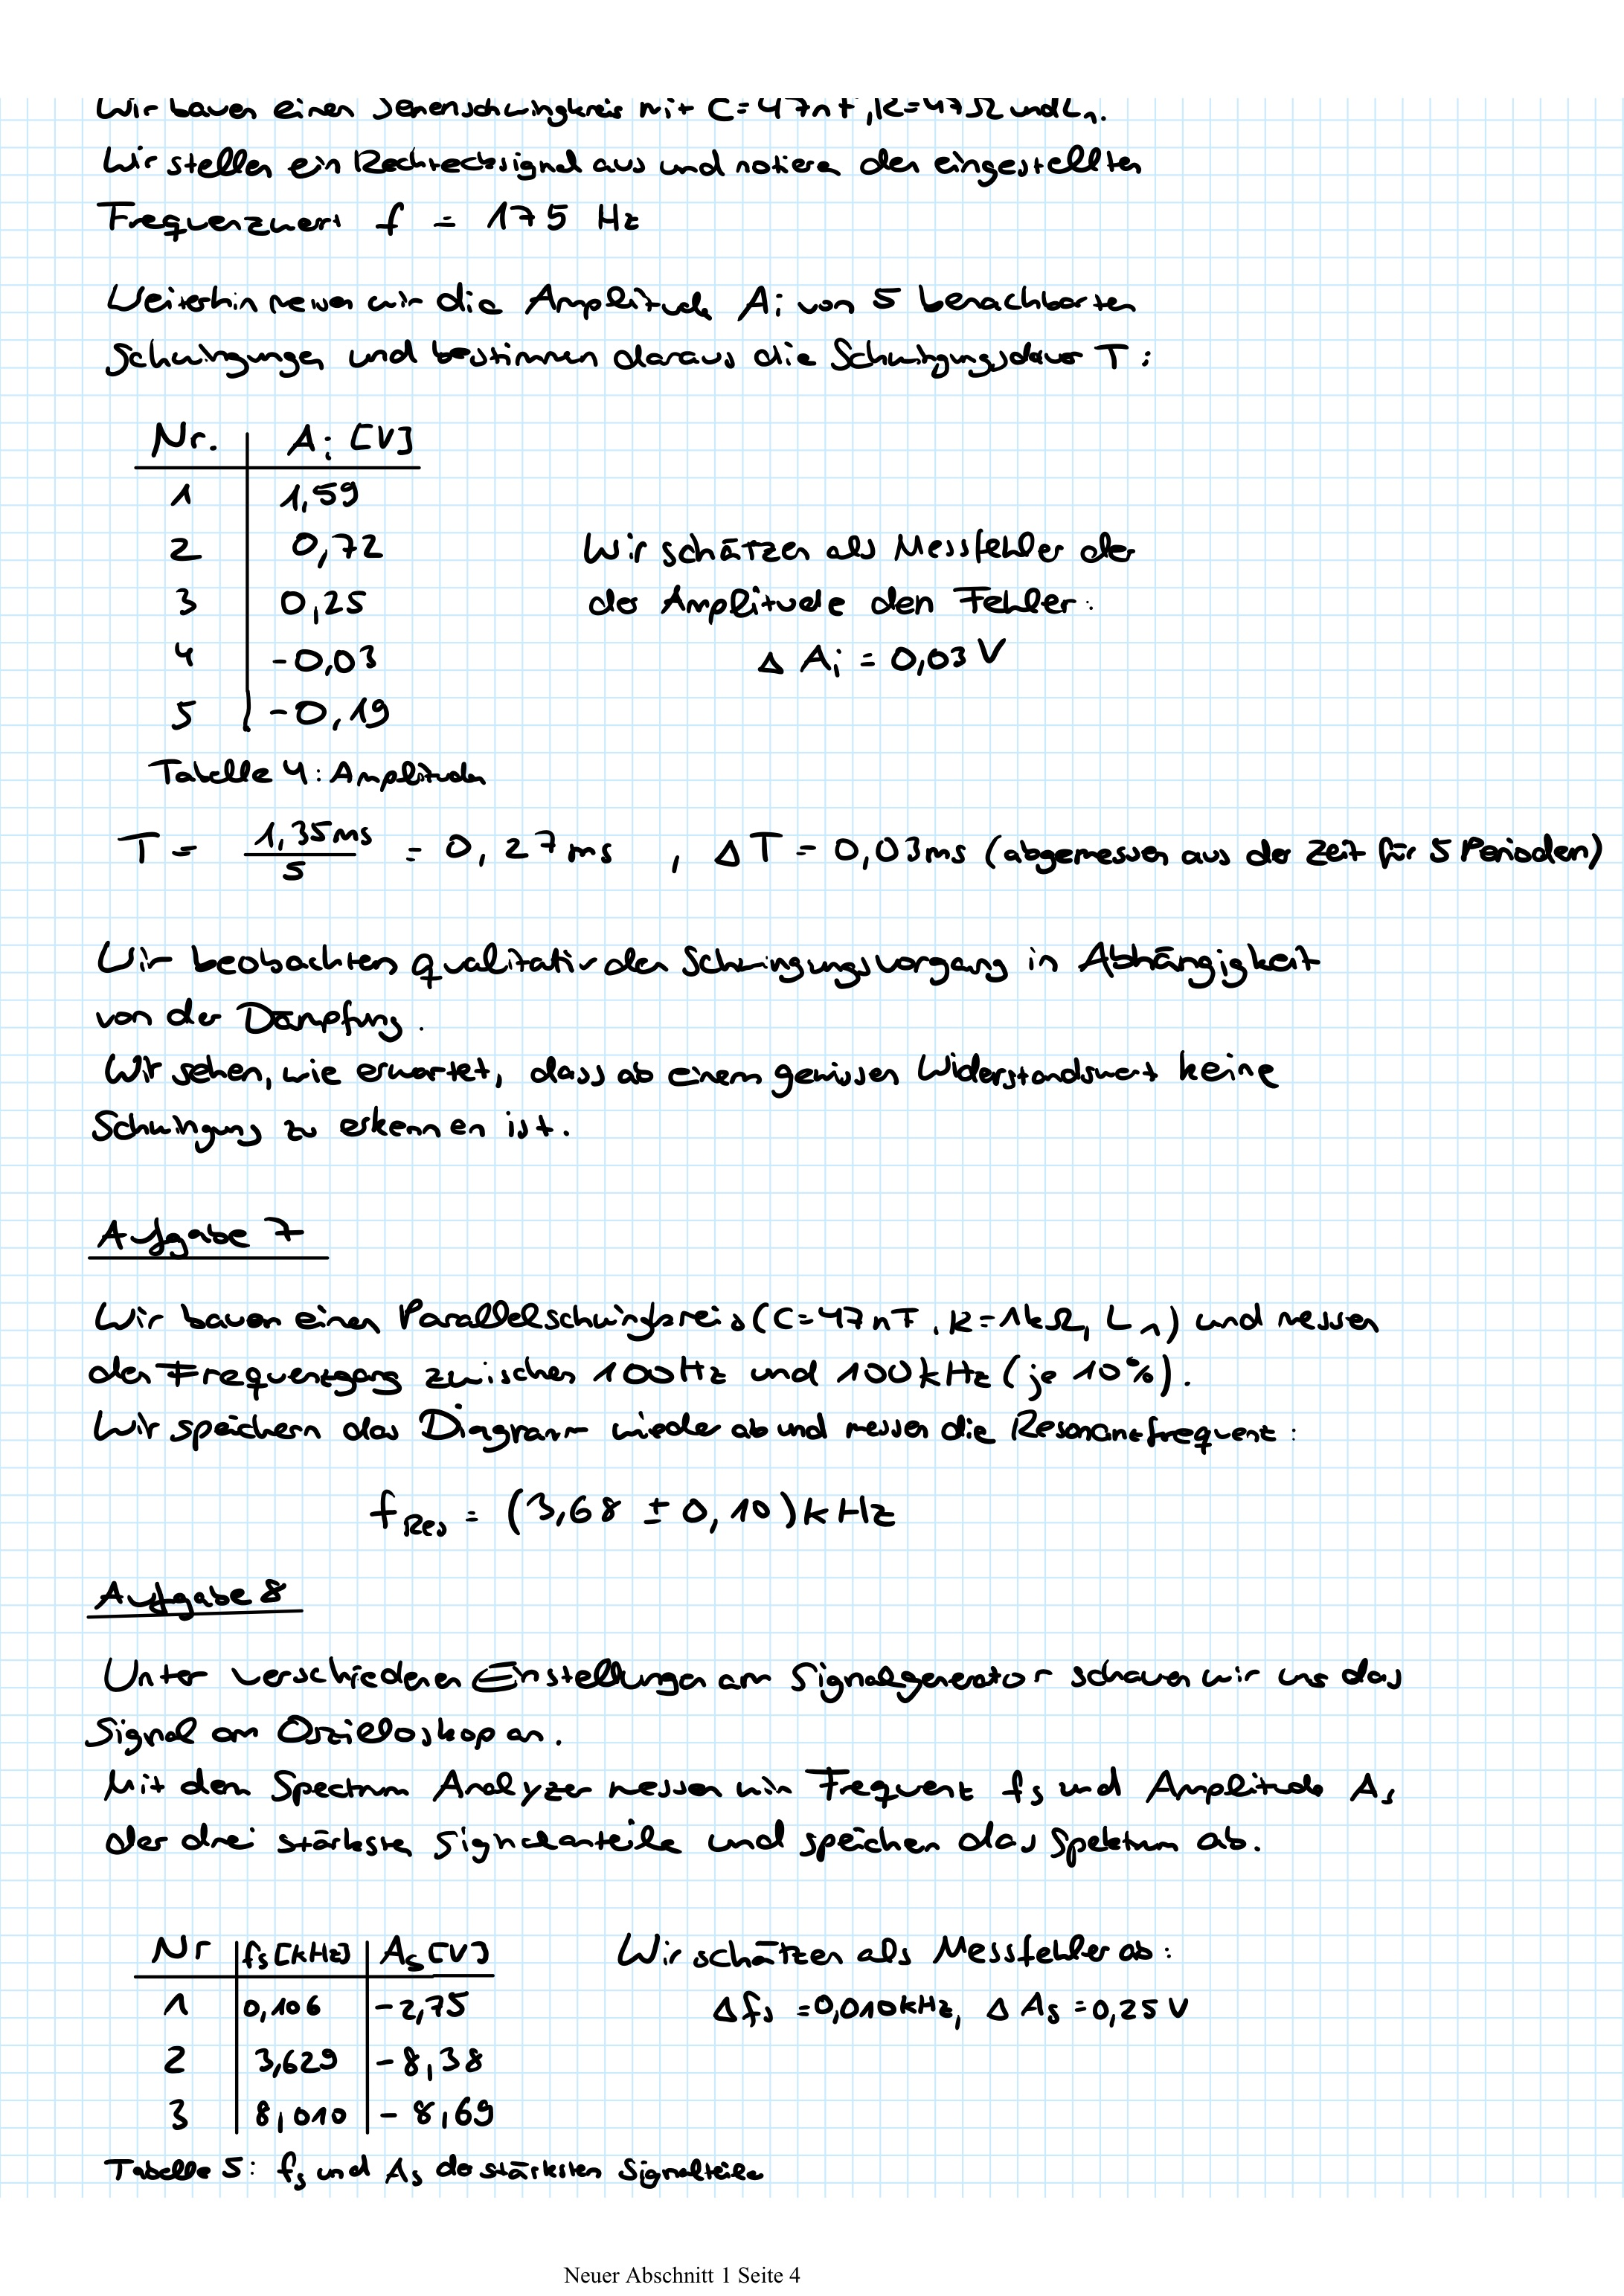
\includegraphics[width=\textwidth]{graphics/mess4.jpg}
\newpage
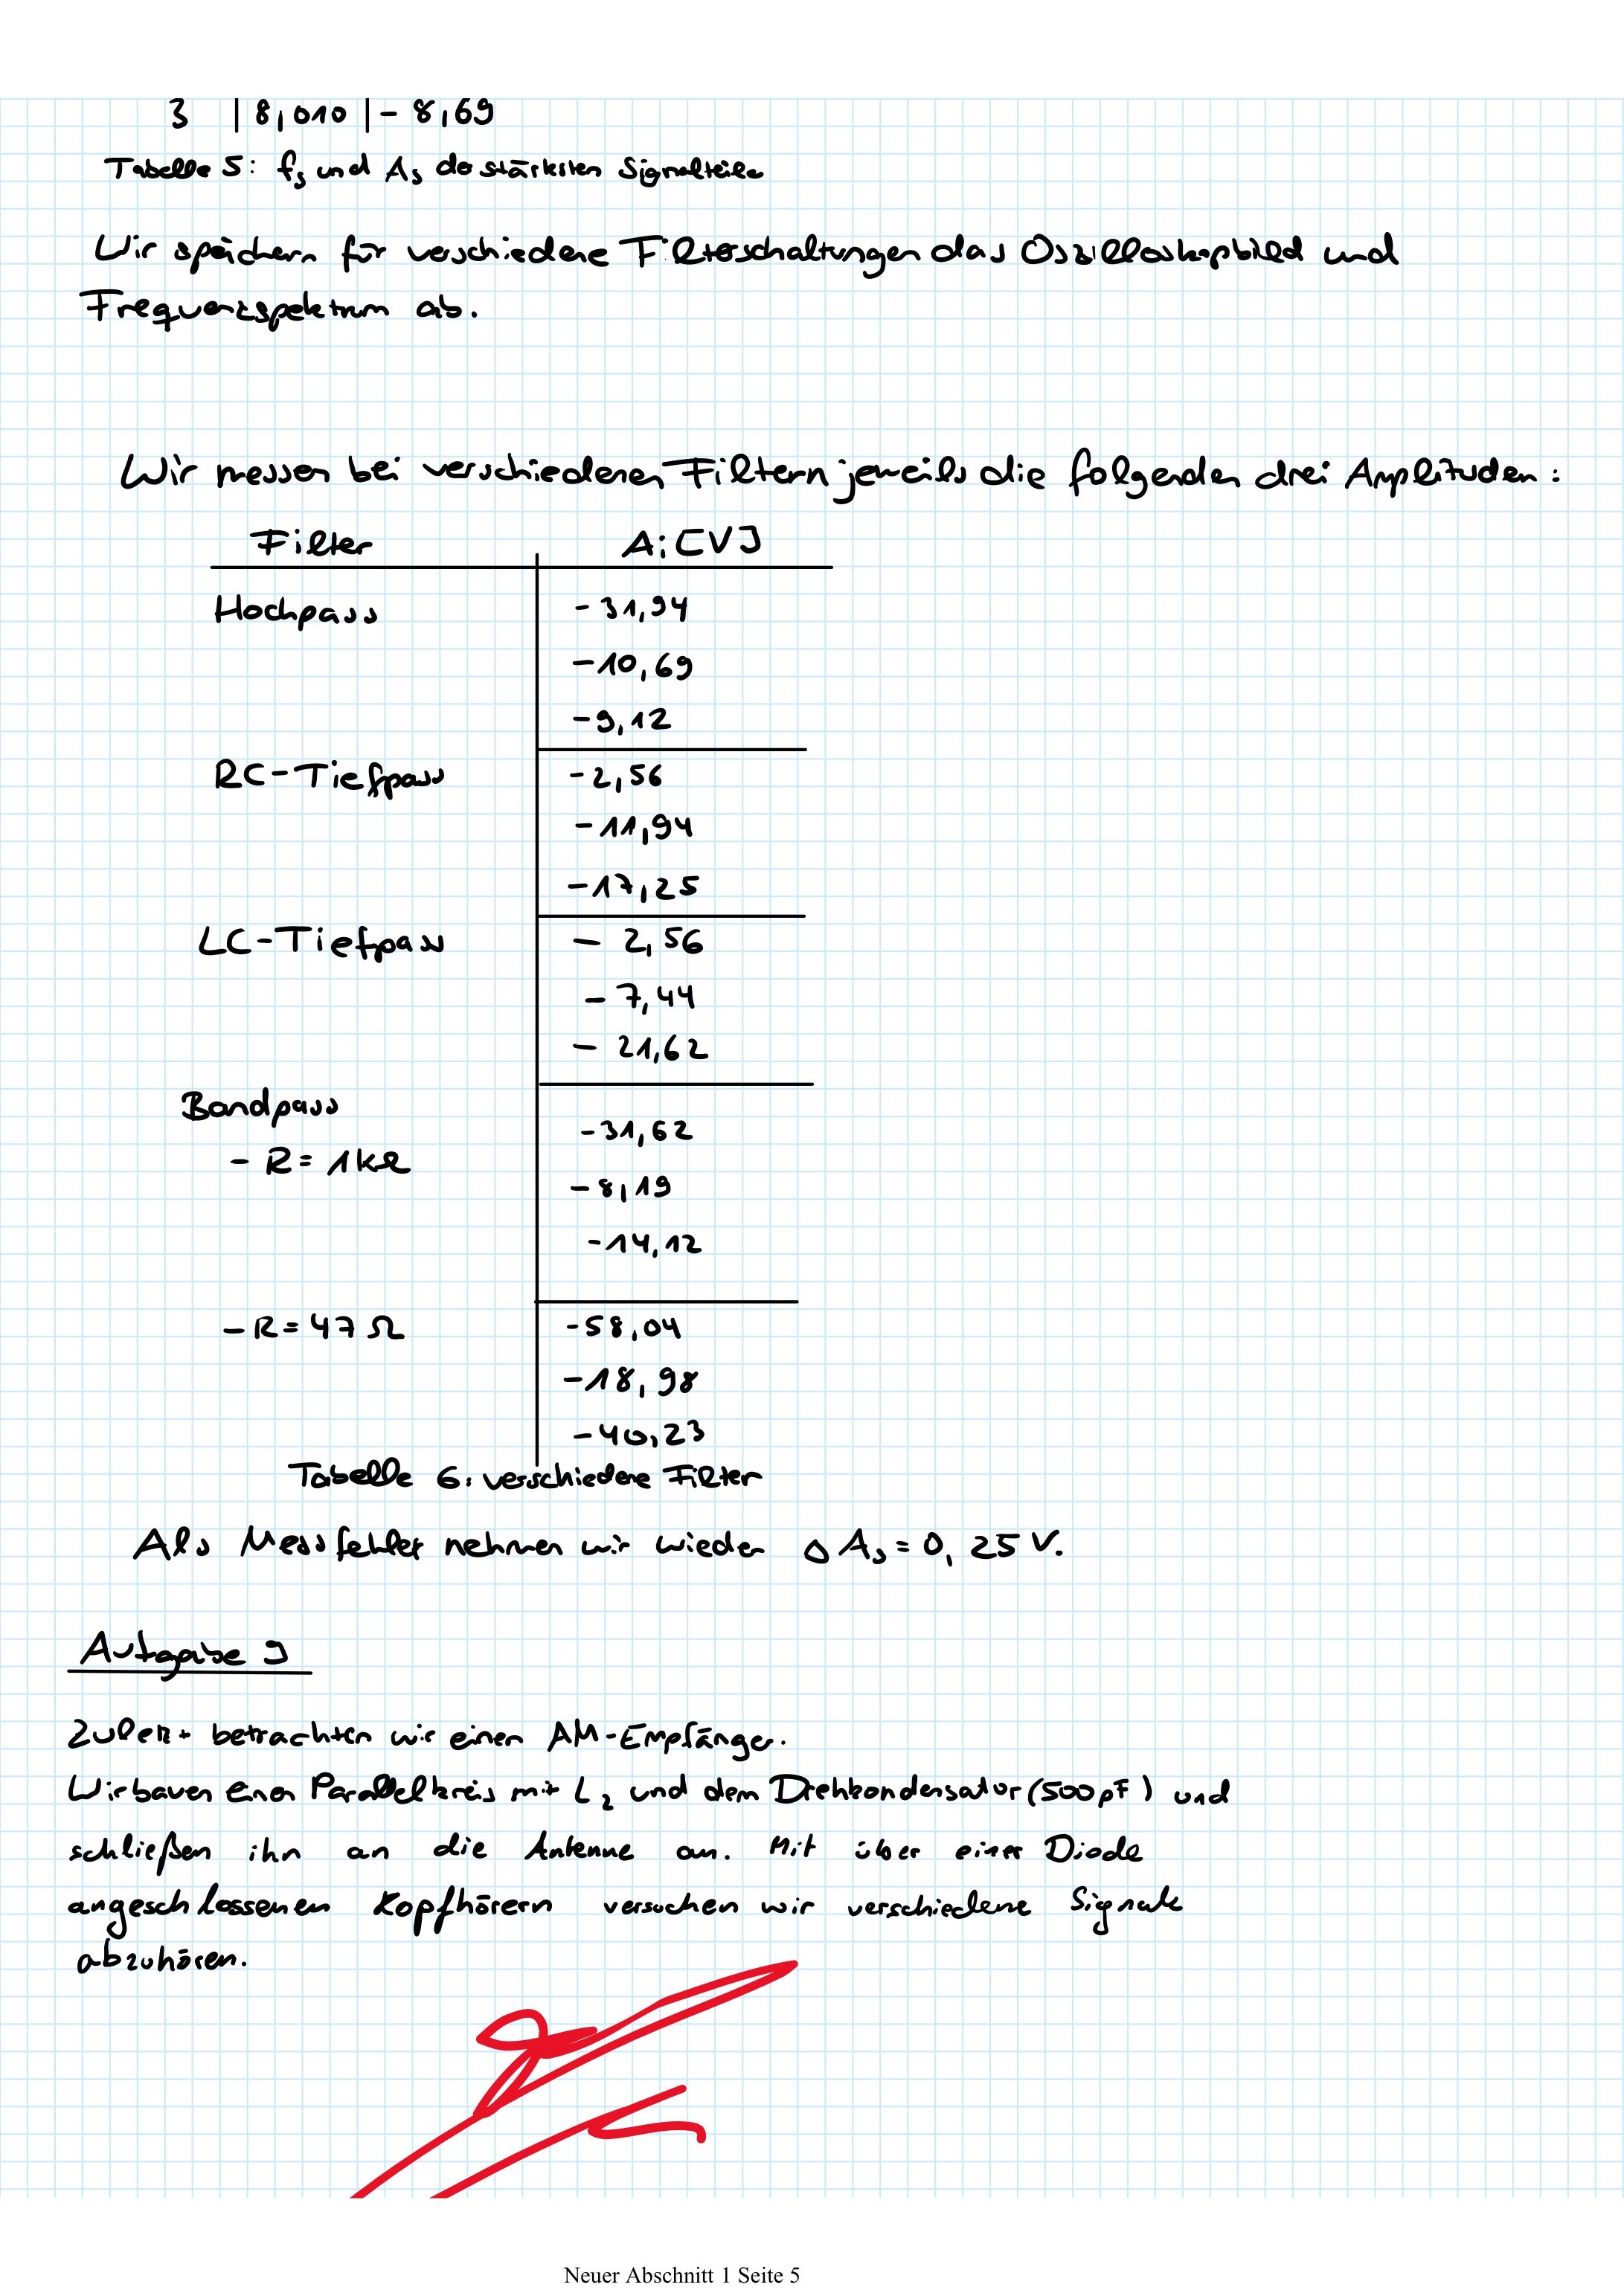
\includegraphics[width=\textwidth]{graphics/mess5.jpg}
\newpage

\addtocounter{table}{6}

\begin{figure}[!p]
  \centering
  \subfloat[R=1k$\Omega$; C=470nF]{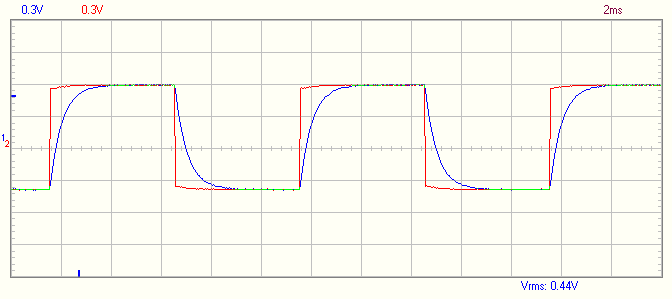
\includegraphics[width=0.7\textwidth]{graphics/teamchopper/A1-1.png}}
  \hfill
  \subfloat[R=10k$\Omega$; C=4,7nF]{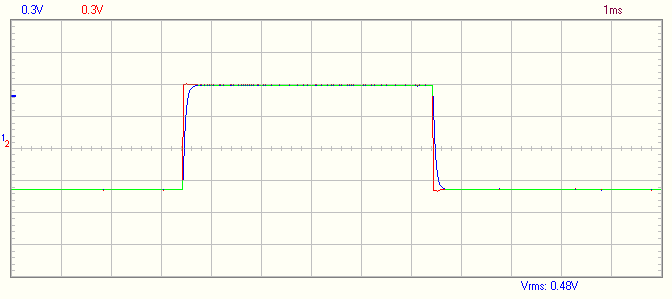
\includegraphics[width=0.7\textwidth]{graphics/teamchopper/A1-2.png}}
  \hfill
  \subfloat[R=1k$\Omega$; C=47nF]{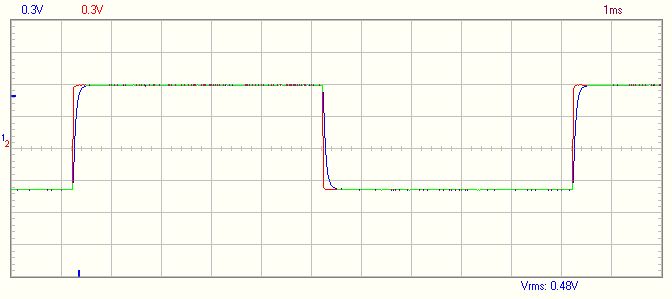
\includegraphics[width=0.7\textwidth]{graphics/teamchopper/A1-3.png}}
  \hfill
  \subfloat[R=1k$\Omega$; C=47nF - C und R getauscht]{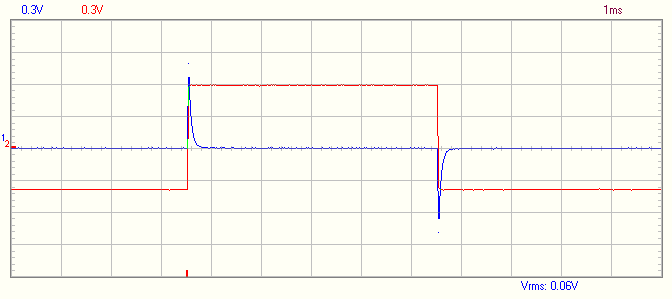
\includegraphics[width=0.7\textwidth]{graphics/teamchopper/A1-tausch_kondenstaor.png}}
  \hfill
  \caption{A1 - RC-Kombination - Rechtecksignal}
  \label{fig:A1_Aufnahmen}
\end{figure}

\begin{figure}[!p]
  \centering
  \subfloat[Gaußsignal]{\includegraphics[width=0.7\textwidth]{graphics/teamchopper/A2-integrator-gauß.png}}
  \hfill
  \subfloat[Rechtecksignal]{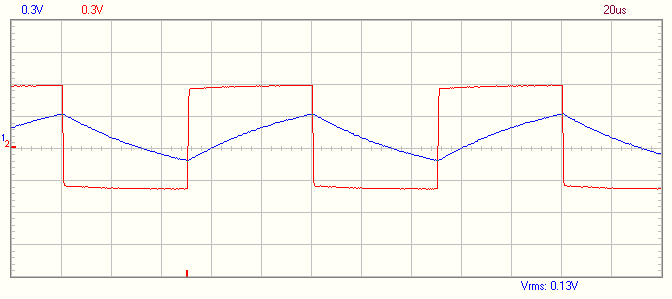
\includegraphics[width=0.7\textwidth]{graphics/teamchopper/A2-integrator-rechteck.png}}
  \hfill
  \subfloat[Sägesignal]{\includegraphics[width=0.7\textwidth]{graphics/teamchopper/A2-integrator-säge.png}}
  \hfill
  \caption{A2 - Integrator}
  \label{fig:A2_Aufnahmen_integrator}
\end{figure}

\begin{figure}[!p]
  \centering
  \subfloat[Gaußsignal]{\includegraphics[width=0.7\textwidth]{graphics/teamchopper/A2-differentiator-gauß.png}}
  \hfill
  \subfloat[Rechtecksignal]{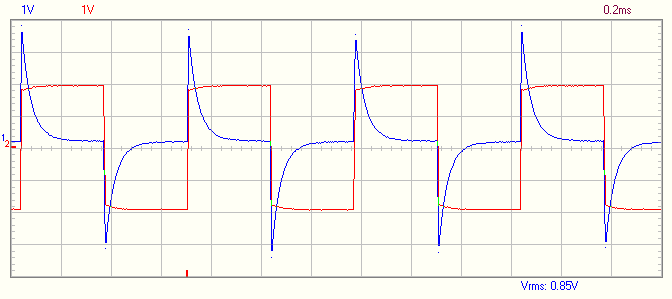
\includegraphics[width=0.7\textwidth]{graphics/teamchopper/A2-differentiator-rechteck.png}}
  \hfill
  \subfloat[Dreiecksignal]{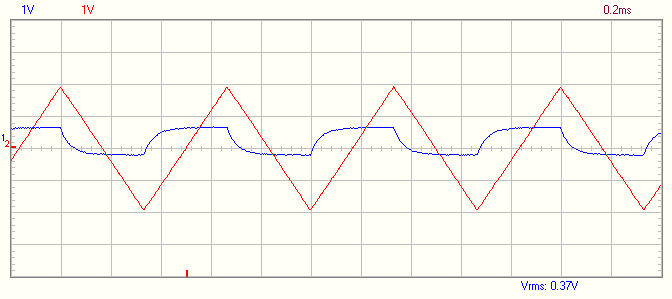
\includegraphics[width=0.7\textwidth]{graphics/teamchopper/A2-differentiator-dreieck.png}}
  \hfill
  \caption{A2 - Differentiator}
  \label{fig:A2_Aufnahmen_differentiator}
\end{figure}

\begin{figure}[!p]
  \centering
  \subfloat[Hochpass]{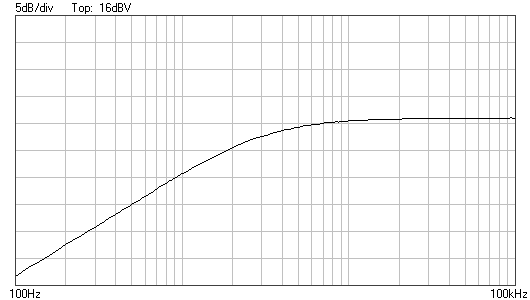
\includegraphics[width=0.9\textwidth]{graphics/teamchopper/A3-hochpass.png}}
  \hfill
  \subfloat[Tiefpass]{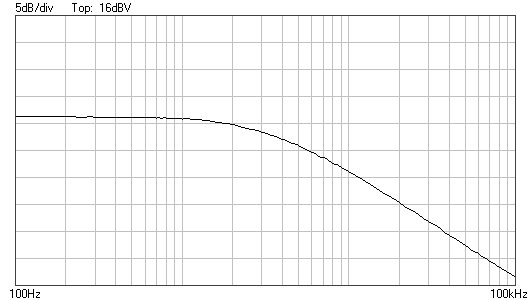
\includegraphics[width=0.9\textwidth]{graphics/teamchopper/A3-tiefpass.png}}
  \hfill
  \caption{A3 - Frequenzgänge Hoch- und Tiefpass}
  \label{fig:A3_Aufnahmen}
\end{figure}

\clearpage
\newpage

\begin{figure}[p]
    \centering
    \resizebox{0.9\textwidth}{!}{
    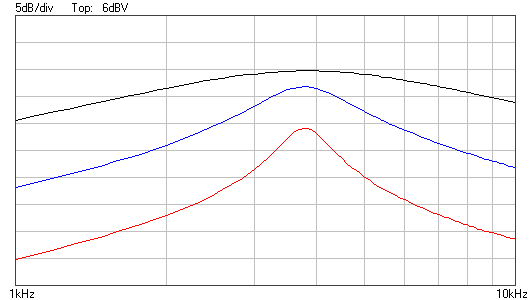
\includegraphics{graphics/teamchopper/A4.png}}
    \caption{A4 - Frequenzgang Serienschwingkreis}
    \label{fig:A4_Aufnahme}
\end{figure}

\begin{figure}[p]
    \centering
    \resizebox{0.9\textwidth}{!}{
    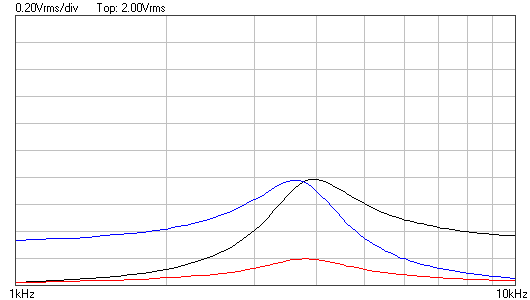
\includegraphics{graphics/teamchopper/A5.png}}
    \caption{A5 - Frequenzgang Resonanzüberhöhung}
    \label{fig:A5_Aufnahme}
\end{figure}

\begin{figure}[p]
    \centering
    \resizebox{0.9\textwidth}{!}{
    \includegraphics{graphics/teamchopper/A6 - gedämpfter schwingkreis.png}}
    \caption{A6 - Gedämpfter Schwingkreis}
    \label{fig:A6_Aufnahme}
\end{figure}

\begin{figure}[p]
    \centering
    \resizebox{0.9\textwidth}{!}{
    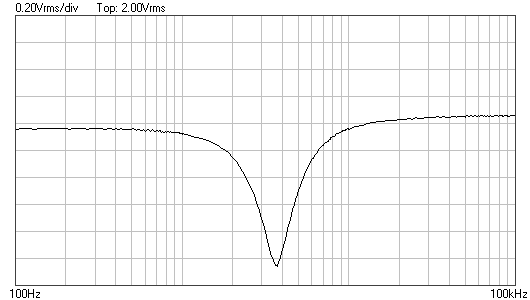
\includegraphics{graphics/teamchopper/A7 - parallel.png}}
    \caption{A7 - Frequenzgang Bandsperre}
    \label{fig:A7_Aufnahme}
\end{figure}

\clearpage
\newpage

\begin{figure}[!p]
  \centering
  \subfloat[Rohes Signal]{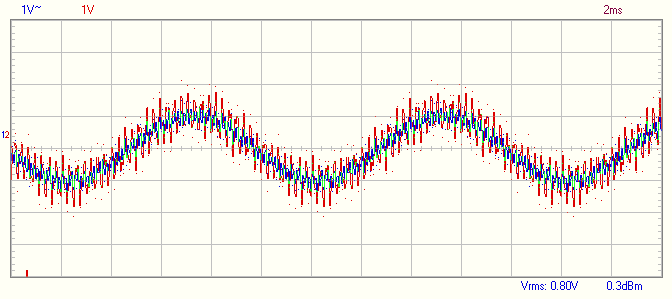
\includegraphics[width=0.49\textwidth]{graphics/teamchopper/A8 - raww.png}}
  \hfill
  \subfloat[Rohes Signal - FFT]{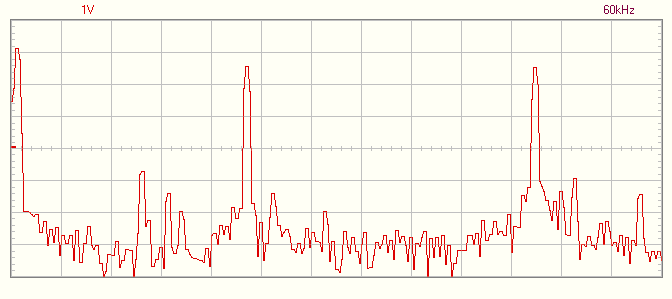
\includegraphics[width=0.49\textwidth]{graphics/teamchopper/A8 - raww - FFT.png}}
  \hfill
  \subfloat[RC-Hochpassfilter]{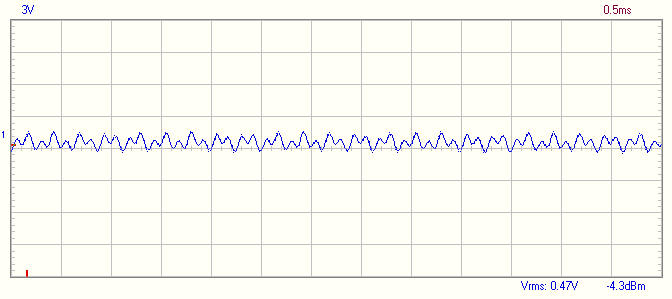
\includegraphics[width=0.49\textwidth]{graphics/teamchopper/A8 - hochpassfilter.png}}
  \hfill
  \subfloat[RC-Hochpassfilter - FFT]{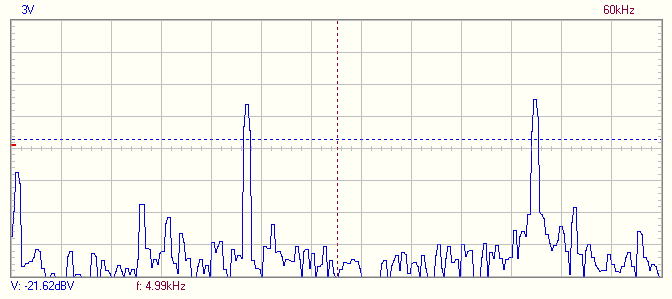
\includegraphics[width=0.49\textwidth]{graphics/teamchopper/A8 - hochpassfilter - fft.png}}
  \hfill
  \subfloat[RC-Tiefpassfilter]{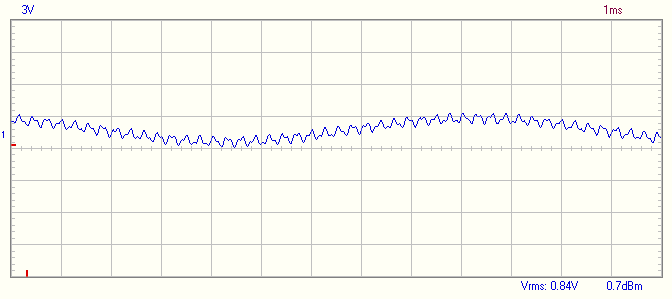
\includegraphics[width=0.49\textwidth]{graphics/teamchopper/A8 - rc-tiefpass.png}}
  \hfill
  \subfloat[RC-Tiefpassfilter - FFT]{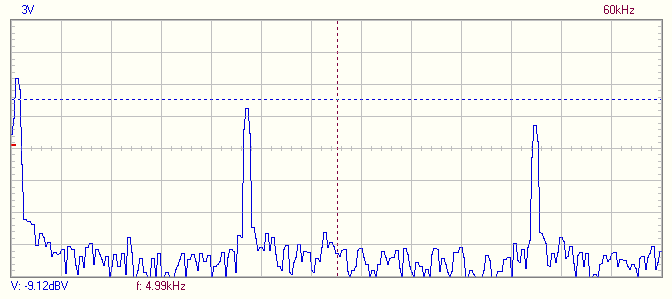
\includegraphics[width=0.49\textwidth]{graphics/teamchopper/A8 - rc-tiefpass - fft.png}}
  \hfill
  \caption{A8 - Signalformung Teil 1}
  \label{fig:A8_Aufnahmen1}
\end{figure}

\begin{figure}[!p]
  \centering
  \subfloat[LC-Tiefpassfilter]{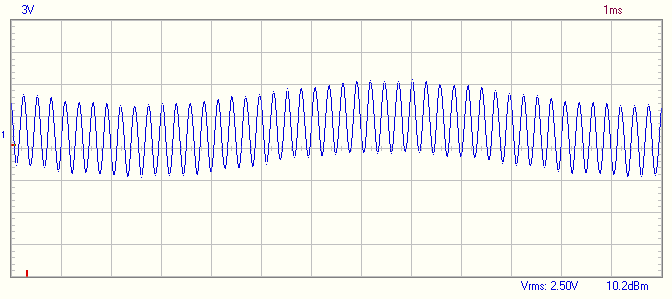
\includegraphics[width=0.49\textwidth]{graphics/teamchopper/A8 - lc-tiefpass.png}}
  \hfill
  \subfloat[LC-Tiefpassfilter - FFT]{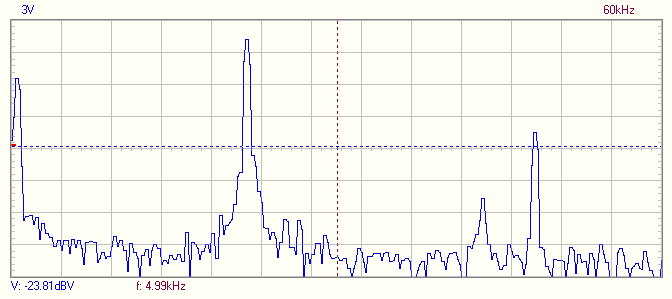
\includegraphics[width=0.49\textwidth]{graphics/teamchopper/A8 - lc-tiefpass - fft.png}}
  \hfill
  \subfloat[Bandpassfilter R=1k$\Omega$]{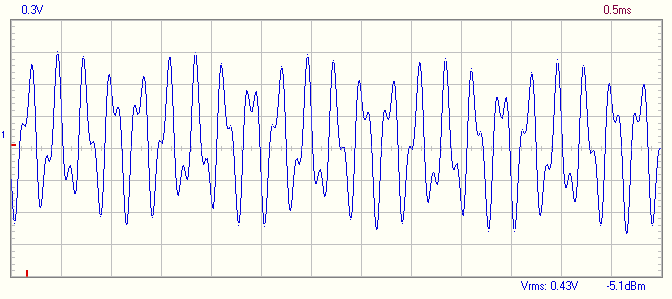
\includegraphics[width=0.49\textwidth]{graphics/teamchopper/A8 - bandpassfilter 1kohm.png}}
  \hfill
  \subfloat[Bandpassfilter R=1k$\Omega$ - FFT]{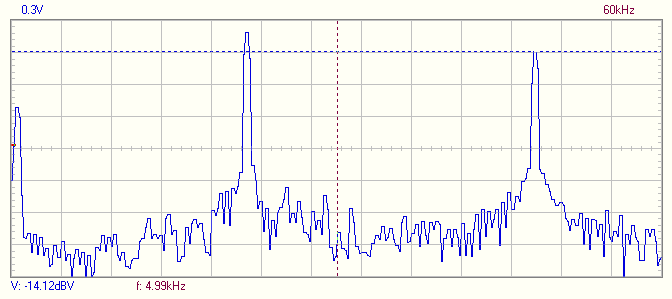
\includegraphics[width=0.49\textwidth]{graphics/teamchopper/A8 - bandpassfilter 1kohm - fft.png}}
  \hfill
  \subfloat[Bandpassfilter R=47$\Omega$]{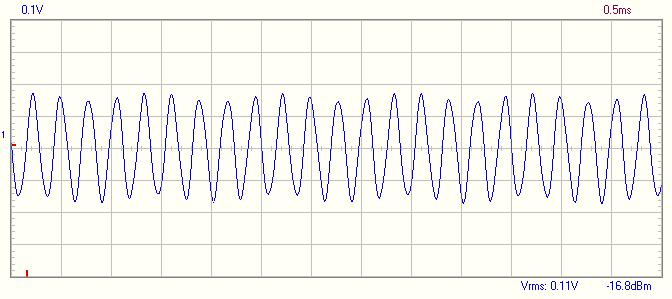
\includegraphics[width=0.49\textwidth]{graphics/teamchopper/A8 - bandpassfilter 47ohm.png}}
  \hfill
  \subfloat[Bandpassfilter R=47$\Omega$ - FFT]{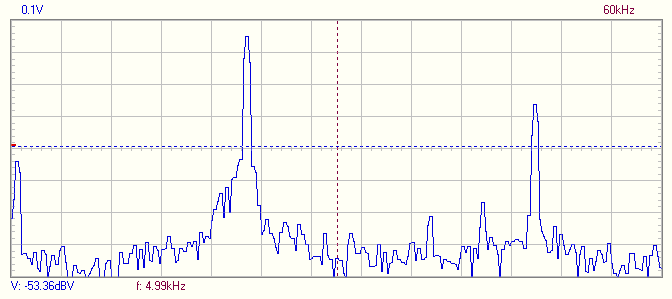
\includegraphics[width=0.49\textwidth]{graphics/teamchopper/A8 - bandpassfilter 47ohm - fft.png}}
  \hfill
  \caption{A8 - Signalformung Teil 2}
  \label{fig:A8_Aufnahmen2}
\end{figure}


\clearpage
\newpage
%-------------------------AUSWERTUNG-------------------------
\section{Auswertung}

In dieser Evaluation werden alle Fehler, sofern keine spezifische Angabe gemacht wird, mithilfe der Gauss'schen Fehlerfortpflanzung berechnet. Dies bedeutet, dass ein Wert $F$, der mit der Formel $f(a_1, ..., a_n)$ berechnet wird, den Fehler $\Delta F$ annimmt:

\begin{equation}
    \Delta F = \sqrt{\sum_n \left( \frac{\partial f}{\partial a_n} \cdot \Delta a_n \right)^2}.
\end{equation}

Des Weiteren erfolgen Signifikanztests von zwei Werten $a$ und $a'$ über die folgende Formel:

\begin{equation}
    \sigma = \frac{|a-a'|}{\sqrt{(\Delta a)^2 + (\Delta a')^2}}.
\end{equation}

Die Auswertung sowie Berechnung erfolgen über das dem Dokument angehängte Python-Programm. Hierbei erfolgen Fits von Funktionen mithilfe der 'curve\_fit'-Funktion des 'SciPy'-Packages und Plots werden mit 'matplotlib' erstellt.

\newpage

\subsection{Zeitkonstanten der RC-Kombinationen}

Wir beginnen und werten die Ergebnisse des ersten Versuchsteils aus. Aus den gemessenen Halbwertszeiten $T_{1/2}$ bestimmen wir die Zeitkonstanten $\tau$ für jede Konfiguration nach Gleichung \ref{eq:E_zeitkonst}. Die Fehler berechnen sich nach Gauß gemäß $\Delta \tau = \Delta T_{1/2} / \ln{2}$ und die Ergebnisse $\tau_{exp}$ sind in Tabelle \ref{tab:A1-Zeitkonst} eingetragen. Ebenso sind die Theoretisch zu erwarteten Zeitkonstanten $\tau_{theo} = R C$ mit Signifikanztests der experimetell bestimmten Werte verzeichnet. Die Fehler der Theoretischen Werte ergeben sich aus den angegeben Toleranzen von 10\% für die Kondensatoren und 5\% für die Widerstände gemäß

\begin{equation}
    \Delta \tau_{theo} = \tau_{theo} \sqrt{0,1^2 + 0,05^2}.
\end{equation}

\phantom{.}

\begin{table}[!h]
    \centering
    %\resizebox{\textwidth}{!}{
    \begin{tabular}{cccccc}
        \hline
        $\bm{C}$ [nF] & $\bm{R}$ [k$\Omega$] & $\bm{f}$ [Hz] & $\bm{\tau_{exp}}$ [10$^{-5}$s] & $\bm{\tau_{theo}}$ [10$^{-5}$s] & $\bm{\sigma}$ \\ \hline
         470 $\pm$ 47 &  1,00 $\pm$   0,05 & 100 & 48 $\pm$ 4 & 47 $\pm$ 5 & 0,09 \\
         4,7 $\pm$ 0,5 & 10,0 $\pm$  0,5 & 100 & 4,75 $\pm$ 0,07 & 4,7 $\pm$ 0,5 & 0,09 \\
         47 $\pm$ 5 &  1,00 $\pm$   0,05 & 100 & 4,96 $\pm$ 0,07 & 4,7 $\pm$ 0,5 & 0,50  \\ \hline
    \end{tabular}%}
    \caption{Experimentelle und theoretische Zeitkonstanten}
    \label{tab:A1-Zeitkonst}
\end{table}

\phantom{.}

Bei den Ergebnissen sind keine signifikanten Abweichungen außerhalb der $3\sigma$-Grenze vorhanden. Dies zeigt, dass die experimentell gemessenen Werte gut zu den aus der Theorie Erwarteten passen, was eine positive Bestätigung der Messergebnisse darstellt.


\clearpage
\newpage

\subsection{RC-Glied als Integrator und Differentiator}

Wir wollen hier kurz auf die aufgenommenen Oszilloskopbilder eingehen, bei denen das RC-Glied als Differentiator und Integrator verwendet wurde. Die Bilder des Integrators sind dem Messprotokoll angehängt in Abbildung \ref{fig:A2_Aufnahmen_integrator} und die des Differentiators in Abbildung \ref{fig:A2_Aufnahmen_differentiator}. 

Beim Integrator ist die rote Kurve jeweils das Eingangssignal und die blaue das Ausgangssignal. Bei allen drei Signalen, ergo bei Gaußsignal, Rechtecksignal und Sägesignal, stimmt der Verlauf der Ausgangskurve gut mit dem aus der Analysis erwarteten Verlauf überein. Die blauen Kurven sind in gleicher Weise periodisch wie die Eingangssignale und weisen die richtigen Merkmale an den richtigen Stellen auf, wie beispielsweise die Knicks an den Kanten des Rechteck- und Sägesignals. 

Ebenso zufriedenstellend sind die Ergebnisse der Differentiatior-Bilder. Auch hier sind die Einganssignale rot und die Ausgangssignale blau. Analog zum Integrator weisen die blauen Kurven die richtigen Verläufe und Merkmale wie Knicks an den richtigen Stellen, auf und passen somit gut zu den theoretisch erwarteten Beobachtungen. 

Bei beiden Betriebsweisen wurden also passende Ergebnisse gefunden welche bestätigen, dass man mit einem RC-Glied tatsächlich Signale integrieren und differenzieren kann.  




\clearpage
\newpage

\subsection{Grenzfrequenzen des Hoch- und Tiefpassfilters}

\subsubsection{Bestimmung aus den Frequenzgängen} \label{chap:A3_frequenzgänge}

Aus unseren aufgenommenen Frequenzgängen des Hoch- und Tiefpasses, zu sehen in Abbildung \ref{fig:A3_Aufnahmen}, wollen wir die Grenzfrequenzen bestimmen. Dazu fitten wir lineare Funktionen an die linear verlaufenden Bereiche der Frequenzgänge an. Zu beachten ist, dass durch die doppellogarithmische Darstellung die Fitfunktionen die Form $y = \alpha \cdot x^\beta$ annehmen. Wir führen also für beide Frequenzgänge die Fits durch, dargestellt in Abbildung \ref{fig:A3-Grenzfrequenz_aus_Frequenzgängen} und erhalten die folgenden Fitfunktionen für den Hochpass:

\begin{equation}
    \begin{split}
        f_{const}(x) &= (0,560 \pm 0,007) \cdot x^{(0,0166 \pm 0,0011)} \\
        f_{lin}(x) &= (3,08 \pm 0,05) \cdot 10^{-4} \cdot x^{(0,9416 \pm 0,0026)}
    \end{split}
\end{equation}

Und die Folgenden für den Tiefpass:

\begin{equation}
    \begin{split}
        g_{const}(x) &= (0,767 \pm 0,008) \cdot 10^{3} \cdot x^{-(0,0196 \pm 0,0016)} \\
        g_{lin}(x) &= (1,43 \pm 0,05) \cdot 10^{3} \cdot x^{-(0,957 \pm 0,004)}
    \end{split}
\end{equation}

Die x-Werte der Schnittpunkte dieser Funktionen sind unsere Grenzfrequenz und berechnen sich mit der oben genannten Fitfunktion folgendermaßen:

\begin{equation}
    x = \exp{ \underbrace{ \left( \frac{\ln \alpha_2 - \ln \alpha_1}{\beta_1 - \beta_2} \right) }_{= \xi}}
\end{equation}

\begin{equation}
    \begin{split}
        \Delta x &= \Delta \xi \cdot \exp{(\xi)} \\
        \Delta \xi &= \xi \sqrt{\left( \frac{\Delta A}{A} \right)^2 + \left(  \frac{\Delta B}{B}  \right)^2} \\ \\
        &\text{mit:} \ \ \ \ \ A = \ln \alpha_2 - \ln \alpha_1 \\
        &\phantom{mit:} \ \Rightarrow \Delta A = \sqrt{\left( \frac{\Delta \alpha_1}{\alpha_1} \right)^2 + \left( \frac{\Delta \alpha_2}{\alpha_2} \right)^2} \\
        &\text{und:} \ \ \ \ \ B = \beta_1 - \beta_2 \\
        &\phantom{mit:} \ \Rightarrow \Delta B = \sqrt{(\Delta \beta_1)^2 + (\Delta \beta_2)^2}
    \end{split}
\end{equation}

So erhalten wir die folgenden Werte für die Grenzfrequenzen von Hoch- und Tiefpass:

\begin{equation}
    \begin{split}
        \bm{f_{g,hp}} &= \bm{(3,34 \pm 0,11)} \textbf{kHz} \\
        \bm{f_{g,tp}} &= \bm{(3,08 \pm 0,17)} \textbf{kHz}
    \end{split}
\end{equation}

Verglichen mit den im Messprotokoll notierten direkt beim Versuch gemessenen Werten von $f_{g,hp} = (3,25 \pm 0,10)$kHz und $f_{g,tp} = (2,99 \pm 0,10)$kHz ergeben sich Sigmaabweichungen von $\sigma_{hp} = 0,60$ und $\sigma_{tp} = 0,45$. Dies sind beide insignifikante Abweichungen, was zeigt, dass das Ablesen der Grenzfrequenz bei dem 1/$\sqrt{2}$-fachen des Maximalwerts und die Methode über den Schnittpunkt der Geraden miteinander verträgliche Ergebnisse liefern und diese somit bestätigen. 


\begin{figure}[!hp]
  \centering
  \subfloat[Hochpass]{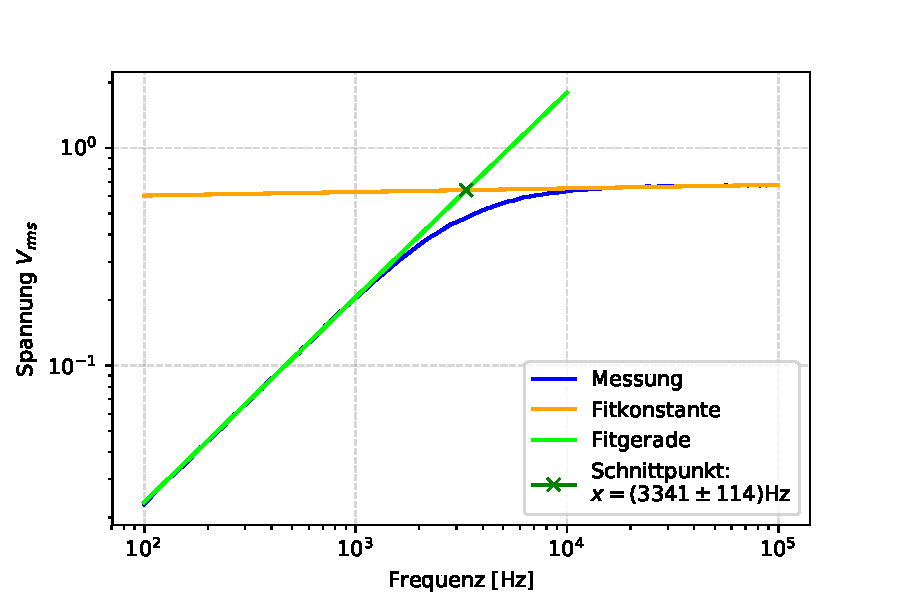
\includegraphics[width=0.9\textwidth]{graphics/plots/A3-hochpass.pdf}}
  \hfill
  \subfloat[Tiefpass]{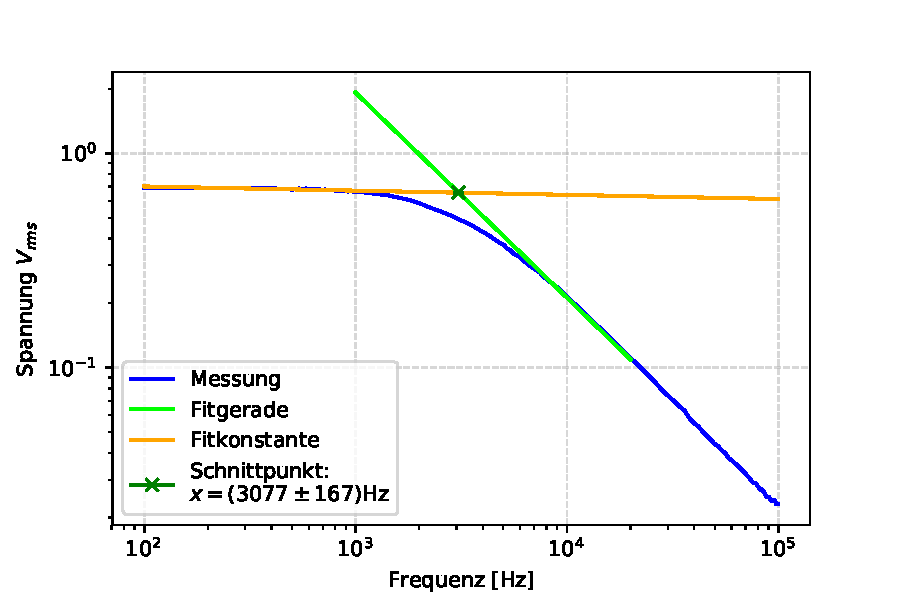
\includegraphics[width=0.9\textwidth]{graphics/plots/A3-tiefpass.pdf}}
  \hfill
  \caption{Grenzfrequenz aus den Frequenzgängen}
  \label{fig:A3-Grenzfrequenz_aus_Frequenzgängen}
\end{figure}





\clearpage
\newpage

\subsubsection{Bestimmung aus dem Phasengang}

Eine weitere Methode zur Bestimmung der Grenzfrequenz folgt aus den aufgenommen Daten des Phasengangs aus Tabelle 2 des Messprotokolls. Indem wir die Phase als Funktion der Frequenz in ein Diagramm eintragen und annehmen, dass wir uns nur im mittleren annähernd linearen Teil des theoretischen Verlaufs befinden, können wir eine Gerade an die Messwerte fitten und den Wert bei einer Phase von 45° als Grenzfrequenz ablesen. Da wir diesmal nur auf der x-Achse eine logarithmische Skala haben nimmt unsere Gerade die Form $y = \alpha \cdot \ln{x} + \beta$ an und unser Fit, zu sehen in Abbildung \ref{fig:A3-Grenzfrequenz_aus_Phasengang} ergibt die folgenden Fitparameter:

\begin{equation}
    \begin{split}
        \alpha &= -(40,2 \pm 0,9) \text{°/Hz} \\
        \beta &= (380 \pm 7) \text{°}
    \end{split}
\end{equation}

Der Wert $x$ bei einer Phase von 45° ergibt sich nun folgendermaßen:

\begin{equation}
    x = \exp{\underbrace{\left( \frac{45^\circ - \beta}{\alpha} \right)}_{= \xi}}
\end{equation}

\begin{equation}
    \begin{split}
        \Delta x &= \Delta \xi \cdot \exp{(\xi)} \\
        \Delta \xi &= \xi \sqrt{\left( \frac{\Delta \alpha}{\alpha} \right)^2 + \left(  \frac{\Delta \beta}{\beta}  \right)^2}
    \end{split}
\end{equation}

Somit erhalten wir hier eine Grenzfrequenz von 

\begin{equation}
    \bm{f_g = (4,1 \pm 1,0)} \textbf{kHz}.
\end{equation}

Beim Vergleich mit den Werten des Messprotokolls ergeben sich hier Abweichungen von $\sigma_{hp} = 0,72$ und $\sigma_{tp} = 0,97$. Diese guten Sigmas sind hauptsächlich dem enormen Fehler der Grenzfrequenz aus dem Phasengang geschuldet. Somit lässt sich zwar sagen, dass insgesamt ein Wert in der ungefähr gleichen Größenordnung rauskommt, diese Methode aber im allgemeinen nicht sehr akkurat ist und gröbere Fehler aufzeigt.

\begin{figure}[!h]
    \centering
    \resizebox{0.9\textwidth}{!}{
    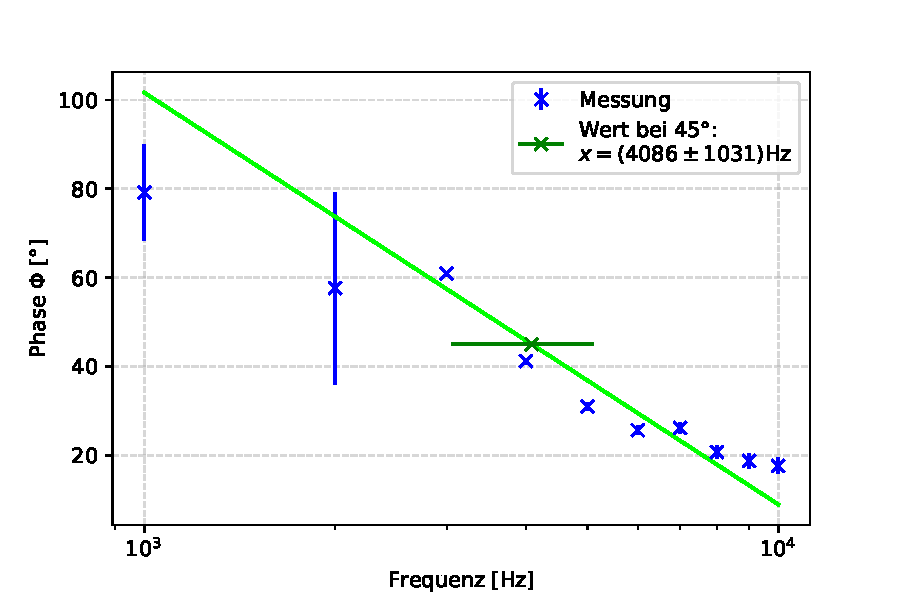
\includegraphics{graphics/plots/A3-phasengang.pdf}}
    \caption{Grenzfrequenz aus dem Phasengang}
    \label{fig:A3-Grenzfrequenz_aus_Phasengang}
\end{figure}

\phantom{.}

\newpage

\subsubsection{Vergleich mit Theoretischen Werten}

Zuletzt berechnen wir erneut theoretischen Werte zum Vergleich für unsere soeben bestimmten Werte der Grenzfrequenz. Die Grenzfrequenz lässt sich folgendermaßen berechnen, wobei die gleichen Tolaranzen für Kondensatoren und Widerstände wie zuvor angenommen werden (C = 47nF; R = 1k$\Omega$):

\begin{equation}
    \begin{split}
        f_{g,theo} &= \frac{1}{2\pi} \frac{1}{RC} \\
        \Rightarrow \Delta f_{g,theo} &= f_{g,theo} \cdot \sqrt{0,1^2 + 0,05^2} \\ \\
        &\Rightarrow \bm{f_{g,theo} = (3,4 \pm 0,4)} \textbf{kHz}
    \end{split}
\end{equation}

Wir vergleichen diesen Wert mit den in Kapitel \ref{chap:A3_frequenzgänge} bestimmten Grenzfrequenzen und erhalten $\sigma_{hp} = 0,35$ und $\sigma_{tp} = 1,01$. Dies sind beides erneut insignifikante Abweichungen, was unsere Ergebnisse positiv bestätigt und zeigt, dass unsere Messung hier gut mit den theoretisch erwarteten Werten übereinstimmt. Ein Vergleich mit der Grenzfrequenz aus dem Phasengang wurde ausgelassen, da dieser auf Grund des bereits diskutierten hohen Fehlers nicht sinnvoll ist.   


\clearpage
\newpage

\subsection{Induktivität und Innenwiderstand} \label{kap:mean_Induktivität}

Zunächst berechnen wir aus den in Tabelle 3 des Messprotokolls notierten Werten die Induktivität der Spule L1 gemäß $L1 = 1/(C \omega^2)$, wobei $\omega = 2 \pi f$ die Kreisfrequenz ist. Somit gilt die folgende Fehlervormel unter Berücksichtigung der 10\%-igen Toleranz der Kondensatoren:

\begin{equation}
    \Delta L1 = L1 \sqrt{\left( 2 \frac{\Delta \omega}{\omega} \right)^2 + 0,1^2}.
\end{equation}

\phantom{.}

\begin{table}[!h]
    \centering
    %\resizebox{\textwidth}{!}{
    \begin{tabular}{ccc}
        \hline
        $\bm{C}$ [nF] & $\bm{\omega}$ [kHz] & $\bm{L1}$ [H]  \\ \hline
         47 $\pm$ 5 & 24,19 $\pm$ 0,19 & 0,036 $\pm$ 0,004 \\
         47 $\pm$ 5 & 23,69 $\pm$ 0,19 & 0,038 $\pm$ 0,004 \\
         47 $\pm$ 5 & 23,88 $\pm$ 0,19 & 0,037 $\pm$ 0,004 \\ \hline
    \end{tabular}%}
    \caption{Berechnung der Induktivität L1}
    \label{tab:A4-L1}
\end{table}

\phantom{.}

Wir erhalten die in Tabelle \ref{tab:A4-L1} dargestellten Ergebnisse, aus denen sich der folgende Mittelwert für die Indiktivität $\overline{L}1$ ergibt:

\begin{equation}
    \bm{\overline{L}1 = (0,037 \pm 0,004)} \textbf{H}
\end{equation}

Der Fehler des Mittelwerts errechnet sich dabei folgendermaßen aus dem statistischen Fehler sowie den Messfehlern:

\begin{equation}
    \begin{split}
        \Delta \overline{L}1 &= \sqrt{\sigma_{std}^2 + \left( \frac{1}{N} \sum_{i=1}^N \Delta L1_i \right)^2} \\
        \text{mit} \ \ \ \sigma_{std} &= \sqrt{\frac{1}{N(N-1)} \sum_{i=1}^N (\overline{L}1 - L1_i)^2}.
    \end{split}
\end{equation}

Des Weiteren möchten wir die bisher unbeachteten Verluste des Schwingkreises durch den Kondensator, die Spule und mögliche andere Effekte qualitativ bestimmen. Aus unseren Messungen der Bandbreite $\Delta \omega = 2 \pi \Delta f$ können wir mit folgender Formel den Gesamtwiderstand $R + R_V$ und somit den Verlustwiderstand $R_V$ aus der Differenz mit dem eingestellten ohmschen Widerstand $R$ bestimmen:

\begin{equation}
    \begin{split}
        R+R_V &= \Delta \omega \cdot L1 \\
        &\Rightarrow \Delta (R+R_V) = \sqrt{(\Delta(\Delta \omega) \cdot L1)^2 + (\Delta \omega \cdot \Delta L1)^2} \\ \\
        R_V &= (R+R_V) - R \\
        &\Rightarrow \Delta R_V = \sqrt{(\Delta (R+R_V))^2 + (0,05 \cdot R)^2} 
    \end{split}
\end{equation}

Wir erhalten somit die in Tabelle \ref{tab:A4-R_V} eingetragenen Ergebnisse.

\phantom{.}

\begin{table}[!h]
    \centering
    %\resizebox{\textwidth}{!}{
    \begin{tabular}{cccc}
        \hline
        $\bm{\Delta \omega}$ [kHz] & $\bm{L1}$ [H] & $\bm{R+R_V}$ [k$\Omega$] & $\bm{R}$ [k$\Omega$]  \\ \hline
        30,85  $\pm$ 0,19 & 0.036 $\pm$ 0.004 &   1,12 $\pm$ 0,11      &  0,12 $\pm$    0,12 \\
          9,36 $\pm$ 0,19 & 0.038 $\pm$ 0.004 &    0,36 $\pm$       0,04 &  0,13 $\pm$ 0,04 \\
          4,96 $\pm$ 0,19 & 0.037 $\pm$ 0.004 &    0,185 $\pm$       0,020 &  0,138 $\pm$  0,020 \\ \hline
    \end{tabular}%}
    \caption{Berechnung der Verlustwiderstände}
    \label{tab:A4-R_V}
\end{table}

\phantom{.}

Es ist kurz anzumerken, dass sich hier für die Werte $R_V$ enorm hohe Fehler ergeben, was im Endeffekt mathematisch begründet ist, da man die Differenz mit dem eingestellten Ohmschen Widerstand nimmt, sich also bei den ersten beiden Fällen der Wert stark verringert, der Fehler aber ungefähr gleich groß bleibt. Dies ist später bei den Signifikanztests zu beachten.

Ebenso können wir den Verlustwiderstand $R_V$ aus den Spannungsdifferenzen der Eingangsspannung $U_E$ und Ausgangsspannung $U_A$ berechnen, wobei der Fehler aus der Toleranz des Widerstands von 5\% abgeschätzt wird: 

\begin{equation}
    \begin{split}
        R_V &= R \cdot \left( \frac{U_E}{U_A} - 1 \right) \\
        &\Rightarrow \Delta R_V = 0,05 \cdot R_V
    \end{split}
\end{equation}

So erhalten wir die in Tabelle \ref{tab:A4-R_V2} dargestellten Ergebnisse, welche direkt über einen Signifikanztest mit den zuvor berechneten verglichen werden. 


\begin{table}[!h]
    \centering
    %\resizebox{\textwidth}{!}{
    \begin{tabular}{ccccc}
        \hline
        $\bm{R}$ [k$\Omega$] & $\bm{U_E}$ [V] & $\bm{U_A}$ [V] & $\bm{R_V}$ [$\Omega$] & $\bm{\sigma}$  \\ \hline
         1,00 $\pm$ 0,05    & 0,65 & 0,61 &   66 $\pm$     3 &    0,45 \\
          0,220 $\pm$ 0,011    & 0,6  & 0,43 &   87 $\pm$     4 &    1,25 \\
           0,0470 $\pm$  0,0024 & 0,51 & 0,18 &   86 $\pm$     4 &    2,53 \\ \hline
    \end{tabular}%}
    \caption{Berechnung der Verlustwiderstände aus den Spannungdifferenzen}
    \label{tab:A4-R_V2}
\end{table}

Es sind zwar gerade so keine signifikanten Abweichungen vorhanden, jedoch sind die Verlustwiderstände hier systematisch kleiner als die zuvor berechneten. Gründe hierfür könnten zum einen die Frequenz- und Stromabhängigkeit des kapazitiven Widerstands bei Wechselspannung sein oder Wärmeverluste in der Spule. Grund für letzteres ist vor allem das ständige Ummagnetesieren im Kern der Spule, was insbesondere bei festen Kernen der Spule Wärme generiert. Beim Kondensator treten vorüberwiegend Verluste im Dielektrikum zwischen den Kondensatorplatten auf. Der ständige Feldwechsel bei Wechselspannung sorgt für einen hohen Energieverlust und bei hohen Frequenzen treten Skinneffektverluste auf, bei denen Hochfrequenzströme Verdrängungseffekte bewirken und den effektiven Leitungsquerschnitt verringern. Letzteres ist somit auch bei allen anderen Bauteilen der Fall. 

All diese Effekte sorgen für verschiedene Verluste und können somit als Erklärung für die beobachteten Unterschiede dienen.   




\clearpage
\newpage

\subsection{Auswertung der Frequenzgänge}

\subsubsection{Erneute Berechnung der Induktivität L1}

Wir berechnen erneut die Induktivität der Spule L1, diesmal aus der in Teil 6 gemessenen Periodendauer $T$, aus der wir zunächst die Kreisfrequenz $\omega = 2 \pi / T$ und anschließend mit der Formel für den gedämpften Schwingkreis, Gleichung \ref{eq:GedämpfterSchwingkreis}, die Induktivität berechnen:

\begin{equation}
    \begin{split}
        L &= \frac{1}{2C\omega^2} + \sqrt{\left( \frac{1}{2C\omega^2} \right)^2 - \frac{R^2}{4 \omega^2}} \\
        &= \frac{1}{2C(2 \pi / T)^2} + \sqrt{\left( \frac{1}{2C(2 \pi / T)^2} \right)^2 - \frac{R^2}{4 (2 \pi / T)^2}}
    \end{split}
\end{equation}

\begin{equation}
    \begin{split}
        \Delta L &= \left\{ \left( \frac{2RT^2}{16 \pi^2 \xi} \Delta R \right)^2 + \ldots \right. \\
        &\phantom{=} + \left( \left[ \frac{T(4\xi - R^2 C)}{16 \pi^2 C \xi} + \frac{T^3}{32 \pi^4 C^2 \xi} \right] \Delta T \right)^2 + \ldots \\
        &\phantom{=} \left. + \left( \left[ \frac{T^2}{8 \pi^2 C^2} + \frac{3 T^4}{128 \pi^4 C^3 \xi} \right] \Delta C \right)^2 \right\}^{1/2} \\ \\
        &\text{mit} \ \ \ \ \ \xi = \sqrt{\frac{T^4}{64 \pi^4 C^2} - \frac{T^2 R^2}{16 \pi^2}}
    \end{split}
\end{equation}

Somit erhalten wir den folgenden Wert:

\begin{equation}
    \bm{L1 = (0,039 \pm 0,010)}\textbf{H}
\end{equation}


Wir vergleichen den Wert für $L1$ mit dem im vorherigen Kapitel bestimmten Mittelwert und erhalten eine Abweichung von $\sigma_{L1} = 0,19$. Dies ist eine insignifikante Abweichung, was die Ergebnisse zwar bestätigt, jedoch ist auch hier zu beachten, dass der Fehler der Induktivität hier etwa 1/3 des Gesamtwertes ist, was die Aussagekraft dieses Wertes etwas anzweifelt.  

\newpage
\subsubsection{Bestimmung des Logarithmischen Dekrements}

Für unsere weiteren Berechnungen müssen wir zunächst das logarithmische Dekrement des Serienschwingkreises bestimmen. Dazu dienen die in Tabelle 4 des Messprotokolls aufgelisteten Amplituden. Normalerweise würde man dieses aus den Verhältnissen der Amplituden berechnen. Da aber bei unseren Amplitudenwerten einige negative Werte auftauchen, höchstwahrscheinlich hat sich hier ein ungewünschter offset der Messwerte eingeschlichen, ist es genauso zielführend eine Exponentialfunktion anzufitten, da die Dämpfunkskonstante $\delta$ des Exponentialverlaufs der Amplitude $A(t)$ uns die Berechnung ermöglicht:

\begin{equation}
    A(t) = A_0 \cdot e^{ - \delta \cdot x } + bkg
\end{equation}

Unser in Abbildung \ref{fig:A4-Dämpfungskonst} dargestellter Fit ergibt:

\begin{equation}
    \bm{\delta = (2,12 \pm 0,16) \cdot 10^{3}} \ \textbf{1/s}
\end{equation}

Ebenso wird die Vermutung vom Anfang bestätigt. Der Fit berechnet einen Hintergrundwert von $bkg=-(0,39\pm0,6)$V, welcher für die Verschiebung nach Unten und somit die teils negativen Werte der Amplitude verantwortlich ist.

Das logarithmische Dekrement $\Lambda$ berechnet sich nun folgendermaßen:

\begin{equation}
    \begin{split}
        \Lambda &= \delta T \\
        \Rightarrow \Delta \Lambda &= \sqrt{(\delta \cdot \Delta T)^2 + (T \cdot \Delta \delta)^2} \\ \\
        &\Rightarrow \bm{\Lambda = 0,57 \pm 0,08}
    \end{split}
\end{equation}

\begin{figure}[!h]
    \centering
    \resizebox{0.9\textwidth}{!}{
    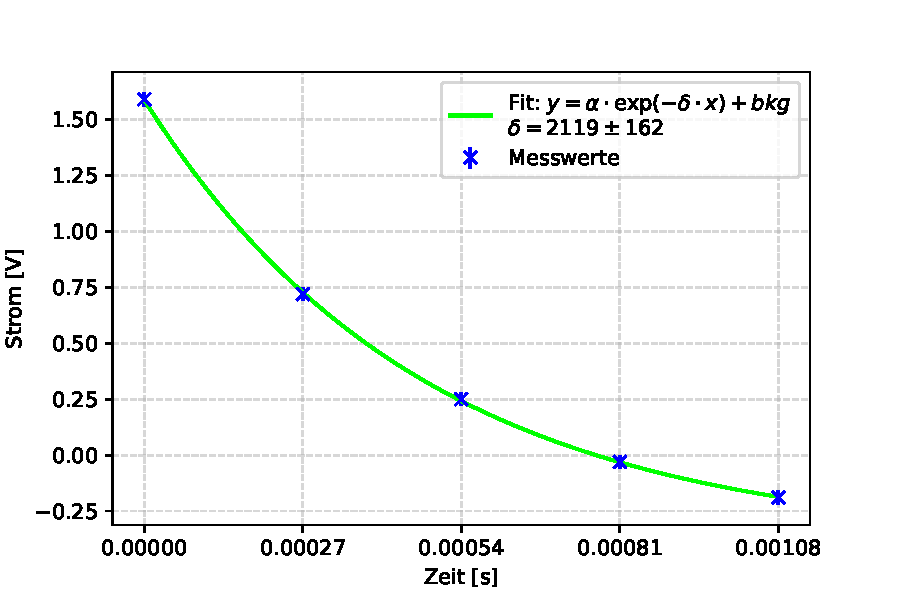
\includegraphics{graphics/plots/A4-logDekr.pdf}}
    \caption{Exponentialfit zur Bestimmung der Dämpfungskonstante}
    \label{fig:A4-Dämpfungskonst}
\end{figure}


\clearpage
\newpage

\subsubsection{Gesamtwiderstand mit dem Logarithmischen Dekrement}

Mithilfe der Dämpfungskonstante können wir nun erneut den Widerstand $R_V$ bestimmen. Dieser ergibt sich wie folgt:

\begin{equation}
    \begin{split}
        R_V &= 2 \delta L \\
        &\Rightarrow \Delta R_V = 2 \sqrt{(L \cdot \Delta \delta)^2 + (\delta \cdot \Delta L)^2}
    \end{split}
\end{equation}

Wir verwenden sie soeben berechnete Induktivität L1 und erhalten somit:

\begin{equation}
    \bm{R_V = (0,17 \pm 0,04) k\Omega} 
\end{equation}

Wir vergleichen diesen Wert zum einen mit dem berechneten Wert aus der Bandbreitenmessung mit gleichem ohmschen Widerstand (220 $\Omega$) und erhalten $\sigma_R = 0,54$ sowie zum Anderen mit dem berechneten Wert aus der Spannungsdifferenz, wobei wir $\sigma_R = 1,78$ erhalten. Hierbei sind beide Abweichungen insignifikant, die zweite ist jedoch etwas erhöht. Erneut lässt sich hier wieder der recht hohe Fehlerwert identifizieren, der sich aufgrund der verwendeten Induktivität L1 ergibt. Man kann aber auch allgemein sagen, dass die Werte selbst ohne Betrachtung der Fehler ungefähr in derselben Größenordnung landen, was an und für sich schonmal eine Bestätigung darstellt.

\subsubsection{Vergleich der Resonanzfrequenzen mit den theoretischen Werten}

Wir beenden diesen Teil der Auswertung, indem wir die in Teil 5 des Messprotokolls aufgenommenen Resonanzfrequenzen $f_R$, $f_C$ und $f_L$ mit den theoretischen Werten vergleichen. Dies geschieht erst am Ende, da dafür die Dämpfungskonstante $\delta$ benötigt wird. Ebenso brauchen wir L1, wofür wir den Mittelwert aus Kapitel \ref{kap:mean_Induktivität} verwenden, sowie die eingestellte Kapazität $C = 47$nF. Der Fehler für $C$ ist die bereits vermehrt genutzte Toleranz von 10\%. Der Wert für $\omega_R$ ergibt sich aus der bereits einmal verwendeten Formel und die anderen beiden folgendermaßen:

\begin{equation}
    \begin{split}
        \omega_R &= \frac{1}{\sqrt{CL}} \\
        &\Rightarrow \Delta \omega_R = \omega_R \sqrt{(0,5 \cdot 0,1)^2 + \left(0.5 \frac{\Delta L1}{L1} \right)^2}
    \end{split}
\end{equation}

\begin{equation}
    \begin{split}
        \omega_C &= \sqrt{\omega_R^2 - 2 \delta^2} \\
        &\Rightarrow \Delta \omega_C = \frac{2}{\omega_C} \sqrt{(\omega_R \cdot \Delta \omega_R)^2 + \left( 2 \delta \cdot \Delta \delta \right)^2}
    \end{split}
\end{equation}

\begin{equation}
    \begin{split}
        \omega_L &= \sqrt{\omega_R^2 + 2 \delta^2} \\
        &\Rightarrow \Delta \omega_L = \frac{2}{\omega_L} \sqrt{(\omega_R \cdot \Delta \omega_R)^2 + \left( 2 \delta \cdot \Delta \delta \right)^2}
    \end{split}
\end{equation}

Die Ergebnisse sind in Tabelle \ref{tab:A6-Vgl_Resonanzfreq} festgehalten, wo auch direkt der Signifikanztest mit den gemessenen Werten umgerechnet in Kreisfrequenzen stattfindet. Wie gut zu erkennen ist ergeben sich hier keine signifikanten Abweichungen. Somit wird unsere Messung bestätigt und die Berechnungen, die in diesem Teil der Auswertungen mit den gemessenen Resonanzfrequenzen durchgeführt wurden, werden zusätzlich auch abgesichert.

\phantom{.}

\begin{table}[!h]
    \centering
    %\resizebox{\textwidth}{!}{
    \begin{tabular}{ccc}
        \hline
        $\bm{\omega_R}$ [kHz] & $\bm{\omega_{R,theo}}$ [kHz] & $\bm{\sigma}$  \\ \hline
         23,88 $\pm$ 0,19 & 23,9 $\pm$  1,7  & 0,02 \\
         22,68 $\pm$ 0,19 & 24 $\pm$  3 & 0,30  \\
         24,76 $\pm$ 0,19 & 24 $\pm$  3 & 0,19  \\ \hline
    \end{tabular}%}
    \caption{Vergleich Resonanzfrequenzen mit Signifiknaztests}
    \label{tab:A6-Vgl_Resonanzfreq}
\end{table}

\phantom{.}

Zuletzt vergleichen wir noch die Resonanzfrequenz aus der Bandsperre in Versuchsteil 7 des Messprotokolls mit dem theoretisch zu erwartenden Wert. Hier gehen wir analog vor wie für $\omega_R$ eben und stellen fest, dass sich durch die verwenden $L1$ sowie die eingestellte Kapazität von $C = 47$nF exakt die gleiche Resonanzfrequenz ergibt wie $\omega_R$. Somit erhalten wir für unsere gemessene Resonanzfrequenz von 

\begin{equation}
    \omega_{\text{Bandsperre}} = (23,1 \pm 0,6) \text{kHz}
\end{equation}

eine Sigmaabweichung von $\sigma_\omega = 0,44$. Dies ist erneut eine insignifikante Abweichung und bestätigt somit, dass auch bei der Aufnahme und Vermessung des Parallelschwingkreises mit Bandsperre miteinander und vor allem mit der Theorie verträgliche Ergebnisse erzielt wurden. 


\clearpage
\newpage

\subsection{Qualitative Analyse der verschiedenen Filterschaltungen}

Hier möchten wir nun noch auf den Versuchsteil 8 eingehen, bei welchem verschiedene Filterschaltungen genutzt wurden, um verschiedene Frequenzanteile eines überlagerten Signals herauszufiltern. Die drei dominanten Frequenzen wurden hierbei immer vermessen und bieten somit die Grundlage der folgenden qualitativen Analyse. Zusätzlich dienen die abgespeicherten Oszilloskopbilder in Abbildungen \ref{fig:A8_Aufnahmen1} \& \ref{fig:A8_Aufnahmen2} als visuelle Bestätigungen.

Beim Hochpass lässt sich deutlich erkennen, dass die ersten beiden Peaks bei niedrigerer Frequenz abgeschwächt wurden und insbesondere der erste eine knapp zehnfach geringere Amplitude aufweist. Hier hat der Hochpass also getan was er sollte und die niedrigeren Frequenzen abgeschwächt während er den dritten Peak bei einer höheren Frequenz fast unverändert lässt. 

Der RC-Tiefpass zeigt das genau umgekehrte Verhalten auf. Hier wurde der Peak bei niedriger Frequenz wie erwartet praktisch gar nicht verringert, während der Peak bei hoher Frequenz auf das knapp doppelte verringert wurde. Der mittlere Peak wurde auch um ein paar Volt sichtbar abgeschwächt. 

Der LC-Tiefpass zeigt den gleichen Effekt wie der RC-Tiefpass, nur deutlich effizienter. Der erste Peak geringer Frequenz blieb wieder unverändert, der höchste Peak wurde aber diesmal bis aufs circa zweieinhalb-fache verringert. Der mittlere Peak hingegen ist etwas höher geblieben als beim RC-Tiefpass was darauf schließen lässt, dass der LC-Tiefpass eine steilere Kante aufweist, ab der Frequenzen abgeschnitten werden. Auch dieses Verhalten wird so von der Theorie bestätigt.

Zuletzt betrachten wir die Beiden Bandpasskonfigurationen. Bei der ersten werden der erste und dritte Peak deutlich unterdrückt, während der mittlere bei ungefähr der gleichen Amplitude bleibt. Dies lässt darauf schließen, dass diese Konfiguration gerade Frequenzen um den mittleren Peak herum durchlässt, während andere rausgefiltert werden. Bei der zweiten Konfiguration hingegen werden alle drei Peaks sichtbar unterdrückt, die beiden äußeren aber deutlich stärker als der mittlere. Somit lässt sich hier interpretieren, dass dieser Bandpassfilter eine schmalere Bandbreite haben muss. Diese Beobachtung wird erneut von der Theorie bestätigt, da hier ein geringerer Widerstand von 47 $\Omega$ im Vergleich zu den vorherigen 1 k$\Omega$ verwendet wurde, was die Trennschärfe des Bandpassfilters erhöht. 

Somit lässt sich festhalten, dass die beobachteten Verhaltensweisen der verschiedenen Filter alle den theoretischen Erwartungen entsprechen und keine größeren Abweichungen festgestellt werden konnten.



\clearpage
\newpage
%---------------PRÄSENTATION DER ENDERGEBNISSE---------------
\section{Zusammenfassung der Endergebnisse}

In diesem Versuch wurden die Grundlagen verschiedenster Schaltkreise bestehend aus ohmschen Widerständen, Kapazitäten und Spulen bei Gleich- und Wechselspannung betrachtet. 

Zuerst bestimmten wir die Zeitkonstanten mehrerer RC-Reihenschaltungen mit unterschiedlichen Bauteilen über eine Halbwertszeitmessung. Beim Vergleich der experimentell bestimmten Werte mit den theoretisch zu erwartenden wurden keine signifikanten Abweichungen festgestellt.

Anschließend wurde das RC-Glied als Integrator sowie Differentiator verwendet und verschiedene Signale quantitativ analysiert. Hier konnte die erwartete Verhaltensweise beobachtet werden, bei der der Verlauf der Ausgangskurven dem integrierten beziehungsweise differenzierten Eingangssignal entsprach und sich mit diesen periodisch korrekt änderte.

Als nächstes bestimmten wir auf verschiedene Weisen die Grenzfrequenzen eines aufgebauten Hoch- und Tiefpassfilters. Aus den ausgenommenen Frequenzgängen wurden die Werte

\begin{equation}
    \begin{split}
        {f_{g,hp}} &= {(3,34 \pm 0,11)} \text{kHz}, \\
        {f_{g,tp}} &= {(3,08 \pm 0,17)} \text{kHz}
    \end{split}
\end{equation}

bestimmt, welche einmal mit dem Wert $f_g = (4,1 \pm 1,0)$kHz bestimmt aus dem Phasengang und darauf mit dem theoretischen Wert $f_{g,theo} = (3,4 \pm 0,4)$kHz aus der Bauteilkonfiguration verglichen wurde, wobei sich immerzu insignifikante Abweichungen ergaben. Dies war jedoch Teils den deutlich erhöhten Fehlern geschuldet. 

Daraufhin verwendeten wir einen Serienschwingkreis zur Bestimmung der Induktivität der verwendeten unbekannten Spule. Eine erste Mittelwertrechnung aus gemessenen Resonanzfrequenzen ergab den Wert 

\begin{equation}
    {\overline{L}1 = (0,037 \pm 0,004)} \text{H}.
\end{equation}

Hierbei fand ebenfalls eine Berechnung des Gesamtwiderstands und Analyse des Verlustwiderrstands des Schwingkreises statt. Zuerst wurden diese mithilfe gemessener Bandbreiten und anschließend aus aufgenommenen Spannungsdifferenzen berechnet. Es ergaben sich hierbei bei der ersten Methode deutlich höhere Werte für den Verlustwiderstand als bei der Zweiten. Der Ursprung dieser Differenz wurde auf die zusätzlichen Verluste in Kondensator und Spule bei verschiedenen Frequenzen und Strömen zurückgeführt.

Anschließend wurde erneut die Induktivität derselben Spule berechnet, diesmal aus einer Periodendauermessung, die den Wert 

\begin{equation}
    {L1 = (0,039 \pm 0,010)}\text{H}
\end{equation}

ergab, welcher insignifikant vom zuvor bestimmten Wert abweicht. Ebenso wurde aus einer Amplitudenmessung die Dämpfungskonstante des gedämpften Schwingkreises sowie das logarithmische Dekrement berechnet:

\begin{equation}
    \begin{split}
        \delta &= (2,12 \pm 0,16) \cdot 10^{3} \ \text{1/s}, \\
        \Lambda &= 0,57 \pm 0,08
    \end{split}
\end{equation}

Damit wurde erneut der Verlustwiderstand des Schaltkreises berechnet, welcher eher mit den zuerst bestimmten Werten übereinstimmte, insgesamt aber dennoch zu beiden Vergleichswerten insignifikante Abweichungen aufwies. 

Daraufhin wurden verschiedenste Messungen von Resonanzfrequenzen aus verschiedensten Frequenzgängen mit den theoretisch berechneten Werten aus der Schaltkreis-Konfiguration verglichen. Hierbei ergaben sich bei allen Werten insignifikante Abweichungen.

Zuletzt wurden verschiedene Hoch-, Tief- und Bandpassfilter qualitativ analysiert. Hierbei ergab der Vergleich der Amplituden der drei dominanten Frequenzen immerzu das erwartete Bild. Bei Hochpässen wurden tiefe und bei Tiefpässen hohe Frequenzen sichtbar abgeschwächt und die Bandpassfilter schwächten alle Frequenzen um die mittlere herum deutlich ab. Ebenso ergaben die Vergleiche verschiedener Filter eines Typs, ergo der Vergleich eines RC- mit einem LC-Tiefpass oder der zweier Bandpassfilter, Sinn und zeigten erwartete Verhaltensweisen.


\newpage
%---------------ZUSAMMENFASSUNG UND DISKUSSION---------------
\section{Diskussion}

Wie in der Zusammenfassung zu sehen konnten größtenteils zufriedenstellende Ergebnisse erzielt werden. Kein Wert überschritt im Vergleich die 3$\sigma$-Grenze und alle qualitativen Beobachtungen und Analysen zeigten erwartete Verhaltensweisen. 

Jedoch wurden in allen Versuchsteilen immer wieder hohe Fehler sichtbar, welche häufig übermäßig dazu beitrugen, dass diese positiven Ergebnisse erzielt werden konnten, wodurch die Aussagekraft und Verlässlichkeit dieser Ergebnisse in Frage gestellt wird. Angefangen bei den angegebenen Toleranzen der Kapazitäten und Widerstände von 10 beziehungsweise 5 Prozent. Diese recht hohen relativen Fehler sorgten von vornherein für eher unsichere theoretische Werte, wenn diese aus den Bauteileigenschaften berechnet wurden. Somit fallen die Signifikanztests hier von vornherein besser aus und dienen daher eher als Abschätzung, ob die Werte aus den Messungen in der richtigen Größenordnung landen. Bauteile, deren Induktivitäten genauer bestimmt werden können, würden hier einen qualitativeren Vergleich erlauben. Allerdings würden sich hier die im Versuch nur nebenbei erwähnten Auswirkungen von beispielsweise Temperaturschwankungen dann auch bemerkbar machen, sodass strenger geregelte Umgebungsbedingungen erforderlich wären, die den Rahmen des Physikalischen Anfängerpraktikums mehr als sprengen würden. Somit sind die hier verwendeten Toleranzen natürlich etwas ungenau, im Kontext dieses Versuchs aber angemessen und ausreichend für den am Ende gezogenen Vergleich der Werte. 

Eine Weitere erwähnenswerte potentielle Fehlerquelle ist der Fakt, dass dieser Versuch über insgesamt zwei Termine, die eine Woche auseinander lagen, durchgeführt wurde. Hierbei konnte von uns nicht garantiert werden, dass wir beim zweiten Termin exakt die gleichen Bauteile verwenden und dass die gleichen Umgebungsbedingungen herrschen wie eine Woche zuvor. Somit können leichte Differenzen zwischen der ersten und zweiten Hälfte des Versuchs auch auf hierbei entstandene Abweichungen zurückzuführen sein, auch wenn bei uns keine auffälligen Messergebnisse dieser Art festzustellen waren. 

Zusammenfassend lässt sich also sagen, dass in diesem Versuch Ergebnisse erzieht wurden, die im Kontext des Physikalischen Anfägerpraktikums durchaus zufriedenstellend sind und der durch den Aufbau bedingten Genauigkeit mehr als genügten. Sowohl die qualitativen als auch die quantitativen Teile ergaben mit der Theorie und untereinander vereinbare Ergebnisse, die für ein grundlegendes Verständnis der Thematik und somit eine angemessene Einführung sorgten. 

 
\newpage
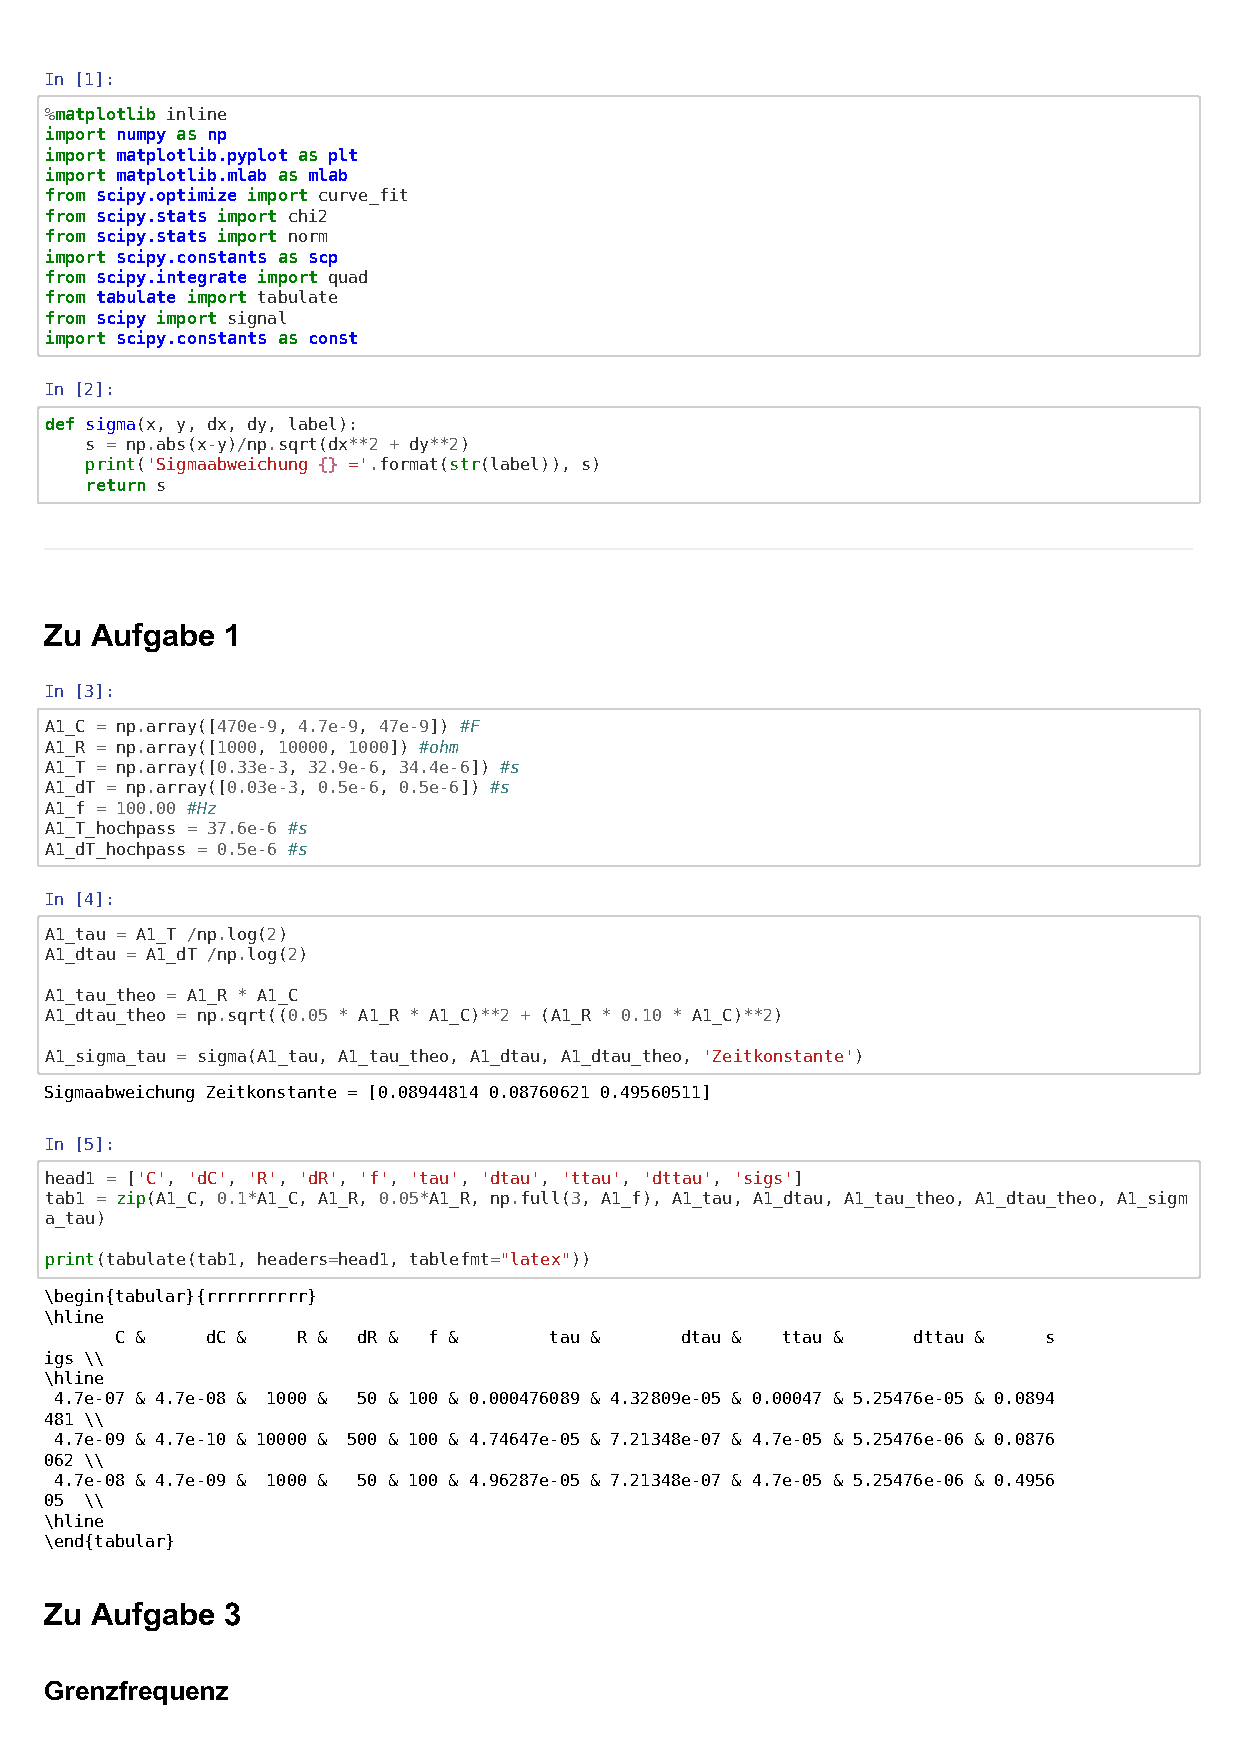
\includepdf[pagecommand=\invisiblesection{Python-Code},scale=0.8,pages=1]{241-Final.pdf}
\includepdf[pagecommand={},scale=0.8,pages=2-last]{241-Final.pdf}

\end{document}

